\documentclass[oneside,a4paper,12pt]{book}
\usepackage[american]{babel}
%\pagestyle{headings}
\frontmatter

%=============================================================================

\usepackage{amsthm}
\usepackage{xspace}
\usepackage{float}
\usepackage{ifthen}
\usepackage{amsbsy}
\usepackage{amssymb}
\usepackage{balance}
\usepackage{booktabs}
\usepackage{graphicx}
\usepackage{rotating}
\usepackage{multirow}
\usepackage{needspace}
\usepackage{microtype}
\usepackage{bold-extra}
\usepackage{geometry}
\usepackage{varioref}
\usepackage{xcolor}
\usepackage{textcomp}
\usepackage{listings}
\usepackage[normalem]{ulem} %emphasize still italic
\usepackage{ucs}
\usepackage{array}

% \usepackage[utf8]{inputenc}
% \usepackage[htt]{hyphenat}
\usepackage{times}
\usepackage{url}
\usepackage{alltt}
\usepackage{amsmath}
\usepackage{xfrac}
\usepackage{subfigure}
\usepackage{appendix}
\usepackage{stmaryrd}   % for the \shortuparrow
\usepackage[utopia]{quotchap}

\usepackage{setspace}
\usepackage[numbers, sort&compress]{natbib}
\usepackage{mdwlist}        % support for better spaced lists
% allows for temporary adjustment of side margins
\usepackage{chngpage}
\usepackage[normalem]{ulem} 

% constants

\newcounter{qcounter}

% commands
\newcommand{\n}{$\cdot$}
\newcommand{\y}{\checkmark}
\newcommand{\subscript}[1]{$_{\textrm{\footnotesize{#1}}}$}
\newcommand{\superscript}[1]{$^{\textrm{\footnotesize{#1}}}$}
\newcommand{\vertical}[1]{\raisebox{-4em}{\begin{sideways}{#1}\end{sideways}}}

\newboolean{showedits}
\setboolean{showedits}{true} % toggle to show or hide edits
\ifthenelse{\boolean{showedits}}
{
       \newcommand{\ugh}[1]{\textcolor{red}{\uwave{#1}}} % please rephrase
       \newcommand{\ins}[1]{\textcolor{blue}{\uline{#1}}} % please insert
       \newcommand{\del}[1]{\textcolor{red}{\sout{#1}}} % please delete
       \newcommand{\chg}[2]{\textcolor{red}{\sout{#1}}{\ra}\textcolor{blue}{\uline{#2}}} % please change
}{
       \newcommand{\ugh}[1]{#1} % please rephrase
       \newcommand{\ins}[1]{#1} % please insert
       \newcommand{\del}[1]{} % please delete
       \newcommand{\chg}[2]{#2}
}


% ============================================================================
% Put edit comments in a really ugly standout display

\usepackage{xcolor}
\usepackage[normalem]{ulem}
\newcommand{\ra}{$\rightarrow$}


% comments \nb{label}{color}{text}
\newboolean{showcomments}
\setboolean{showcomments}{true}
\ifthenelse{\boolean{showcomments}}
    {\newcommand{\nb}[3]{
        {\colorbox{#2}{\bfseries\sffamily\scriptsize\textcolor{white}{#1}}}
        {\textcolor{#2}{\sf\small$\blacktriangleright$\textit{#3}$\blacktriangleleft$}}}
     \newcommand{\version}{\emph{\scriptsize$-$Id$-$}}
%	 \newcommand{\ugh}[1]{\textcolor{red}{\uwave{#1}}} % please rephrase
%	 \newcommand{\ins}[1]{\textcolor{blue}{\uline{#1}}} % please insert
%	 \newcommand{\del}[1]{\textcolor{red}{\sout{#1}}} % please delete
%	 \newcommand{\chg}[2]{\textcolor{red}{\sout{#1}}{\ra}\textcolor{blue}{\uline{#2}}} % please change
	 \newcommand{\chk}[1]{\textcolor{ForestGreen}{#1}} % changed, please check
	}
    {\newcommand{\nb}[3]{}
     \newcommand{\version}{}
	\newcommand{\chk}[1]{} % changed, please check
	}

% ============================================================================
% Make quotes be italic
\renewenvironment{quote}
    {\list{}{\rightmargin\leftmargin}%
     \item\relax\begin{it}}
    {\end{it}\endlist}

\newcommand{\ttimes}{\ensuremath{\times}}

%=============================================================================

\newcommand{\needlines}[1]{\Needspace{#1\baselineskip}}

% source code
\usepackage{xcolor}
\usepackage{textcomp}
\usepackage{listings}
\definecolor{source}{gray}{0.9}
\lstset{
	language={},
	% characters
	tabsize=3,
	upquote=true,
	escapechar={!},
	keepspaces=true,
	breaklines=false,
	alsoletter={:},
	breakautoindent=true,
	columns=fullflexible,
	showstringspaces=false,
	basicstyle=\footnotesize\ttfamily,
	% background
	frame=single,
    framerule=0pt,
	backgroundcolor=\color{source},
	% numbering
	numbersep=5pt,
	numberstyle=\tiny,
	numberfirstline=true,
	% captioning
	captionpos=b,
	numberbychapter=false,
	% formatting (html)
	moredelim=[is][\textbf]{<b>}{</b>},
	moredelim=[is][\textit]{<i>}{</i>},
	moredelim=[is][\uline]{<u>}{</u>}}
\newcommand{\ct}{\lstinline[backgroundcolor=\color{white},basicstyle=\footnotesize\ttfamily]}
\newcommand{\lct}[1]{{\small\tt #1}}


%----------------------------------------------------------------------------
% references
\newcommand{\tabref}[1]{\hyperref[{tab:#1}]{Table~\ref*{tab:#1}}}
\newcommand{\figref}[1]{\hyperref[{fig:#1}]{Figure~\ref*{fig:#1}}}
\newcommand{\secref}[1]{\hyperref[{sec:#1}]{Section~\ref*{sec:#1}}}
\newcommand{\lstref}[1]{\hyperref[{lst:#1}]{Listing~\ref*{lst:#1}}}
\newcommand{\charef}[1]{\hyperref[{cha:#1}]{Chapter~\ref*{cha:#1}}}
%----------------------------------------------------------------------------

% abbreviations
\tracingcolors 4
\setcounter{tocdepth}{3}
\setcounter{secnumdepth}{3}
\newcommand{\ie}{\emph{i.e.,}\xspace}
\newcommand{\eg}{\emph{e.g.,}\xspace}
\newcommand{\etc}{\emph{etc.}\xspace}
\newcommand{\etal}{\emph{et al.}\xspace}


\newcommand{\newevenside}{
	\ifthenelse{\isodd{\thepage}}{\newpage}{
	\newpage
        \phantom{placeholder} % doesn't appear on page
	\thispagestyle{empty} % if want no header/footer
	\newpage
	}
}

\def\stretchfactor{1}
\newcommand{\mychapter}[1]{\setstretch{1}
    \chapter{#1}\setstretch{\stretchfactor}}

%----------------------------------------------------------------------------
\newcommand{\lessSpace}{\vspace{-1em}}
\DeclareGraphicsExtensions{.pdf,.png}
\graphicspath{{images/}}
\newcommand{\fig}[4]{
	\begin{figure}[#1]
		\centering
		\includegraphics[width=#2\textwidth]{#3}
		\lessSpace
		\caption{\label{fig:#3}#4}
	\end{figure}}

% ===========================================================================

%:CONFIGURE THIS

\newcommand{\thesistitle}{Cryptographic APIs}
\newcommand{\thesisauthor}{Sophie Gabriela Pfister}
\newcommand{\thesisauthorOrigin}{Bern, Switzerland}
\newcommand{\thesisleiter}{Prof.\ Dr.\ Oscar Nierstrasz}
\newcommand{\thesisasst}{Dr.\ Mohammad Ghafari, Mohammadreza Hazhirpasand}
\newcommand{\thesisurl}{http://scg.unibe.ch/}
\newcommand{\thesissubtitle}{Evaluating the Usability of Java Cryptography Architecture}
\newcommand{\thesisdate}{31. Dezember 2021}

% ===========================================================================

\usepackage[ colorlinks=true, urlcolor=black, linkcolor=black,
			citecolor=black, bookmarksnumbered=true, bookmarks=true,
			plainpages=false,
			pdftitle={\thesistitle}, pdfauthor={\thesisauthor},
			pdfsubject={\thesissubtitle}, pdfpagelabels]{hyperref}

\newcommand{\hrref}[2]{\hyperref}
% ===========================================================================
% ===========================================================================

\hypersetup{
    colorlinks=true,
    linkcolor=black,
    filecolor=magenta,      
    urlcolor=blue,
    }

% D O C U M E N T
% % % % % % % % % % % % % % % % % % % % % % % % % % % % % % % % % %
\begin{document}

% T I T L E
% % % % % % % % % % % % % % % % % % % % % % % % % % % % % % % % % %
\begin{titlepage}  
  \begin{center}  
  
  \begin{figure}[t]  
  \vspace*{-2cm}        % to move header logo at the top 
  \center{
\includegraphics[scale=0.5]{logos/UNI_Bern.png}}
  \vspace{1.2in}     
  \end{figure}

    \thispagestyle{empty}
    
    {\bfseries\Huge \thesistitle \par
    \Large \vspace{0.1in} \thesissubtitle \par}

    \vspace{0.3in} 
    \LARGE{\textbf{Bachelor Thesis} \\}
    \vspace{0.4in}

    {\Large \thesisauthor \par from \par \thesisauthorOrigin}
    
    \vspace{0.3in}
    {\Large Philosophisch-naturwissenschaftlichen Fakult\"{a}t \\
            der Universit\"{a}t Bern \par}
    \vspace{0.3in}
    {\Large \thesisdate \par}
    \vspace{0.3in}
    %Leiter der Arbeit: \par
   {\Large \thesisleiter} \par
      {\Large \thesisasst} \par
   \vspace{0.1in}
    {\Large Software Composition Group \par Institut f\"{u}r Informatik \par University of Bern, Switzerland \par}
  

  %\vspace{0.5in}
 
 

  \end{center}

\end{titlepage}


% A B S T R A C T
% % % % % % % % % % % % % % % % % % % % % % % % % % % % % % % % % %
\chapter*{\centering Abstract}
\begin{quotation}
\noindent 
% Background
Recent research revealed for a wide range of cryptography libraries that they lack usability. 
Developers therefore misused them and produced insecure applications.
A commonly observed source for obstacles was lacking documentation quality.
Programmers consult other resources (\ie Stack Overflow) if they do not find the required information or code examples in the official documentation.
% Aims & Methods
\par
In this context, we aimed for an investigation on API level to further clarify developer's obstacles.
We focused on symmetric encryption related APIs from Java Cryptography Architecture (JCA) library, in particular the \lstinline|Cipher| class.
We analyzed the content of 150 threads from Stack Overflow to identify the issues programmers faced when working with these APIs as well as common forms of API misuse causing security risks.
We also sought links between these problems and JCA's documentation by formulating questions for each issue and seeking the answers in the documentation.
% Results & Conclusions
\par
We observed that most of the identified issues related to the generation of parameters (\ie keys) or instantiating a \lstinline|Cipher| object (\ie specifying encryption mode).
About 20\% of issues were discussed regarding security.
However, only 24 threads did not contain any potential security risks.
The identified risks mainly related to the use of unsafe encryption modes and constant/static values as key or initialization vector.
We were able to reduce the issues and security risks to 64 questions.
Most of them ($\sim$84\%) were at least partly covered by the documentation.
We concluded that most issues and cases of misuse could have been prevented if the original poster had read and understood the documentation.
However, JCA's documentation spreads over several documents and finding the required piece of information might therefore be difficult.
Additionally, programmers might lack the required domain knowledge and find documentation hard to understand.
As we revealed several JCA-specific obstacles relating to the documentation or the library design of JCA, we believe that future research should continue evaluating cryptography libraries on API level.\\
\end{quotation}
\clearpage


% C O N T E N T S 
% % % % % % % % % % % % % % % % % % % % % % % % % % % % % % % % % % % % % % % %
\tableofcontents

\mainmatter
%%%%%%%%%%%%%%%%%%%%%%%%%%%%%%%%%%
%%%% NEW CHAPTER %%%%%%%%%%%%%%%%%%%%%
%%%%%%%%%%%%%%%%%%%%%%%%%%%%%%%%%%

% === I N T R O D U C T I O N ===
\chapter{Introduction}
\label{cha:Introduction}
% === Relevance of Cryptography  & Cryptographic APIs + Issues ===
Cryptography is a fundamental part of our digital world. 
It provides techniques to ensure confidentiality, authenticity, and integrity of information. 
Yet, Buchanan described the internet as an unsafe place \cite{buchanan2017}. 
He complained that too little security was implemented in the services and protocols used. 
He insisted that "the next generation of the Internet [...] must be built in a trustworthy way" (Buchanan, 2017, \cite{buchanan2017}, p. 1).\\
In practice, we witness a large number of vulnerabilities found in various software and protocols each year.\footnote{\href{https://www.exploit-db.com}{https://www.exploit-db.com}}
One of the disastrous weakness types is the ones concerning cryptography. 
Although there exist a great number of cryptography libraries for building secure applications by providing services such as hashing, symmetric, and asymmetric encryption, a series of recent studies have indicated that software developers have difficulty using cryptography correctly.
Hazhirpasand \etal analyzed 489 open source Java projects and found that only 2 of them were completely secure \cite{hazhirpasand2020}.\\
\par
One of the leading issues is that cryptography libraries lack usability.
This issue has been studied in a number of well-known cryptography libraries.
The results showed that libraries often do not support auxiliary tasks (\ie Mindermann \etal \cite{mindermann2018}),  that they are not abstract enough (\ie Nadi \etal \cite{nadi2016}), and that they lack documentation quality (\ie Mindermann \etal \cite{mindermann2018}, Nadi \etal \cite{nadi2016}, Patnaik \etal \cite{patnaik2019}).
Similarly, the results of Acar \etal imply that unusable cryptography libraries do not only prevent developers from writing functional code but also lead to the emergence of security vulnerabilities since developers are more likely to misuse APIs \cite{acar2017}.
What's more, a good documentation is a strong predictor for both, functional and secure code.
Acar \etal emphasized the importance of having an official documentation, which contains secure examples "to keep developers from searching for unvetted, potentially insecure alternatives" (2017, \cite{acar2017}, p.167).\\

% === Project Goals & Research Questions ===
\par
We believe that still some areas, such as context of API usability, documentation usability, API misuse and unsafe code, need closer investigations. 
Therefore, for the three aforementioned areas, we are interested to address the following research questions:
\begin{enumerate}
	\item What issues do programmers face when implementing symmetric encryption using Java Cryptography Architecture?
	\item What security risks can be found in code and advice shared on Stack Overflow referring to the implementation of symmetric encryption scenarios Java Cryptography Architecture?
	\item To what extent are these issues linked to missing or inadequate documentation?
\end{enumerate}

Since different cryptography libraries have different API design, it may manifest various and scattered types of issues if we had studied more than one cryptography libraries on Stack Overflow. 
As a result, we focused on one library (\ie Java Cryptography Architecture) and one use case (\ie symmetric encryption) to gain a deeper understanding of the issues, which provides us with more details compared to previous research that focused on a more general level.
The Java Cryptography Architecture (JCA) is the default cryptography API for Java developers and acquired FIPS-140 standards issued by the National Institute of Standards and Technology (NIST) to specify the requirements for cryptography libraries and modules. \footnote{\href{https://nvlpubs.nist.gov/nistpubs/FIPS/NIST.FIPS.140-3.pdf}{FIPS-140-3}}\\

% === Methodology ===
\par
To answer our research questions, we analyzed 150 threads from Stack Overflow where at least one issue related to our scope was discussed.
We used three queries and computed the sample size per query proportional to the number of posts returned by it.
We also selected half of the sample from the newest threads and the other half from the most popular ones.
To answer the first research question, we identified the issues the person asking the question (original poster) was facing and categorized them regarding technical aspects that had been implemented incorrectly or requirements that had not been met.
To answer the second research question, we checked the same sample for rule violations based on a predefined set of security rules for symmetric encryption scenarios.
To answer the third research question, we derived a set of prioritized questions from the previous findings and sought their answer in the documentation of JCA library.
We also took notes regarding documentation quality in general.\\

% === Results ===
\par
Regarding the first research question, we observed that most of the discussed issues referred to generating algorithm parameters (\ie key, initialization vector) (24.2\%), and the \lstinline|Cipher.getInstance(...)| method (22.8\%).
Many errors were caused by developers failing to correctly configure the
dependencies between different properties involved in encryption (\ie encryption mode - padding, algorithm - key size) (27\%). 
Some programmers even used different properties or parameters for encryption and decryption (15.1\% of all issues).
We concluded that these developers lacked the domain knowledge to properly use a low-level cryptography library such as JCA.
Some developers also struggled with the API design of JCA, especially the dependency from providers (\ie default behavior) and the high prevalence of method overloads.\\
\par
Regarding the second research question, we found that programmers frequently used unsafe encryption modes (ECB, CBC). 
75.3 \% of all original posters\footnote{author of the question post in a thread} made use of one of these modes.
They also utilized static values for keys (28.7\%) and initialization vectors (16.0\%).
Other original posters did not implement password based key derivation in a secure way (7.3\%).
They used a weak password (6.7\%), static salt (4.7\%), too few iterations for key derivation\footnote{$< 1,000$} (4\%), short salt\footnote{$< 64$ bits}(2\%), and reused passwords (2\%).
The answer posts contained much fewer security risks. 
Only 27\% of all accepted answers had security risks in their code snippets.
Most of them were inherited from the question post as the person answering the question focused on producing functioning code without thinking of security.\\
\par
Regarding the third research question, we observed that most of the derived questions were covered by the documentation (84.4\%), especially those with higher priorities.
We concluded that most of the issues could have been prevented if the original poster thoroughly read and understood the documentation.
However, an answer might be hard to find since the documentation spreads over several documents (\ie API documentation \cite{javaxCrypto}, Reference Guide \cite{javaReferenceGuide}, Standard Algorithm Name Specification \cite{javaStandardAlgorithmName}).
Additionally, the results from the first and second research questions implied that some programmers lacked domain knowledge.
The documentation might be hard to understand for them.
We considered 27.8\% of the answers as unclear or incomplete.\\
Among the unanswered questions, 70\% targeted cryptography or software security in general.
We observed that JCA documentation did not provide links to resources for comprehensible information about these topics.
It however links the specifications for most algorithms, but the most popular symmetric encryption algorithm, AES, is missing.
Additionally, specifications might be hard to read if one has not a mathematical / technical background.\\

% === Thesis Structure ===
\par
In this thesis, we first present the state of research in chapter \ref{cha:RelWo}. 
In chapter \ref{cha:Method}, we describe the methodical approaches of our study. 
We explain and interpret our results in chapter \ref{cha:Results}.
Chapter \ref{cha:Conclusion} includes the conclusion, limitations, and conductive thoughts.
In the "Anleitung zum Wissenschaftlichen Arbeiten" (chapter \ref{cha:AWI}), we provide and explain a best-practice example for password based encryption using AES-GCM.

% === R E L A T E D   W O R K ===
\chapter {Related Work}
\label{cha:RelWo}


% === Usability ===
\section{API Usability}
\label{cha:ApiUsability}
One of the most popular definitions for usability is by ISO 92411-11:1998: "the extent to which a product can be used by specified users to achieve specified goals with effectiveness, efficiency and satisfaction in a specified context of use" (ISO 9241-11, \cite{iso1998}, p.2).
Although the definition is very precise, it does not explain how to measure the usability of a product.\\
\par
Past research on (API) usability approached the topic in different ways and the literature is therefore heterogeneous.
Some researchers focused rather on programmers' needs and defined guidelines and heuristics to describe what a usable API should look like. 
Zibran conducted a meta analysis on API usability literature and described a set of 22 specific guidelines \cite{zibran2008}.
He considered an API as usable if it was "(1) easy to learn, (2) easy to remember, (3) easy write client code, (4) easy to interpret client code, and (5) difficult to misuse" (2008, \cite{zibran2008}, p. 256).\\
Other researchers approached the problem from the perspective of software metrics.
Rama \& Kak proposed 8 metrics for API usability referring to method overloads and name confusion, method grouping, parameter list complexity and consistency, thread safety, and documentation \cite{rama2015}.
Scheller \& Kühn even defined an extensible framework to measure interface complexity automatically \cite{scheller2015}.\\
Another approach was to focus on the concept of usability and redefine it more precisely.
Alonso-Ríos \etal developed a detailed taxonomy \cite{alonso2010}.
Starting from usability, they organized a wide range of attributes in a hierarchy.\\

\par
Mosquiera-Rey \etal combined several approaches \cite{mosqueira2018}.
They extended the usability model by Alonso-Rìos \etal with the context of use and mapped existing guidelines for API usability to the model's attributes.
The first level attributes of these taxonomies are shown in figure \ref{fig:ApiUsability}.
They identified and described a total of 45 heuristics for API usability.
\begin{figure}[h]
\centering
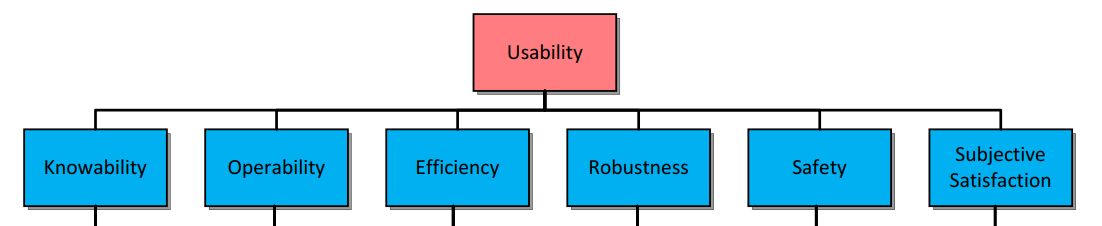
\includegraphics[width=0.65\textwidth]{ApiUsability}
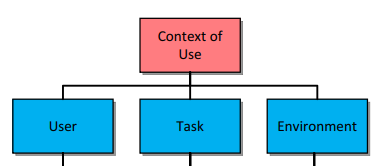
\includegraphics[width=0.33\textwidth]{ContextOfUse}
\caption{First Level Attributes of Usability and Context of Use Taxonomies (Mosquiera-Rey \etal, 2018, \cite{mosqueira2018}, p. 49 ff.)}
\label{fig:ApiUsability}
\end{figure}

% Documentation Usability
\section{Usability Criteria for Documentation}
\label{cha:DocQuality}
Mosquiera-Rey \etal located documentation quality within the \emph{Knowability} attribute of an API \cite{mosqueira2018}.
They defined this property as the extent a programmer can "understand, learn, and remember how to use the system" (Mosquiera-Rey \etal, 2018, \cite{mosqueira2018}, p. 48).
They described three documentation related heuristics:
\begin{itemize}
	\item Documentation should not contain irrelevant information such as meta data or obsolete and redundant comments.
	\item Documentation should contain code samples for key scenarios.
	\item Documentation should identify deprecated methods, explain why these are deprecated, and propose alternatives.
\end{itemize}

Robillard asked developers what they struggled with most when they had to learn a new API \cite{robillard2009}.
Their answers identified missing or unclear documentation as a major obstacle.
Robillard concluded that API documentation must be complete and provide example code.
Additionally, it should support a wide range of usage scenarios, include relevant design elements, and be organized in a convenient way.\\

\newpage
% Recommendations for Crypto Documentation
\par
Mindermann \etal who evaluated the usability of rust cryptography libraries also made recommendations how to improve the usability of such libraries and their documentation \cite{mindermann2018}. 
These were more specific for the cryptographic context.
A good documentation for a cryptography API should additionally
\begin{itemize}
	\item link to comprehensible resources that explain cryptographic concepts.
	\item mention closely related keywords (\ie block cipher mode of operation, cipher mode, encryption mode).
	\item describe in which scenarios an algorithm should be used.
	\item warn from weaknesses and vulnerabilities (\ie unsafe algorithms that are supported for legacy).
	\item explain all parameters.
	\item give advice when there are multiple options and explain the differences between them.
\end{itemize}

\newpage
% Crypto API Usability
\section{Usability of Cryptography Libraries}
\label{cha:CryptoApi}

Green \& Smith defined ten principles regarding the usability and security of cryptography libraries \cite{green2016} .
Their key idea was that security-related functionalities should be integrated into non-cryptographic APIs such that regular programmers\footnote{without cryptography expertise} did not have to deal with cryptography APIs at all.
The entire set of principles is shown in figure \ref{fig:Princip}\\
\begin{figure}[h]
\centering
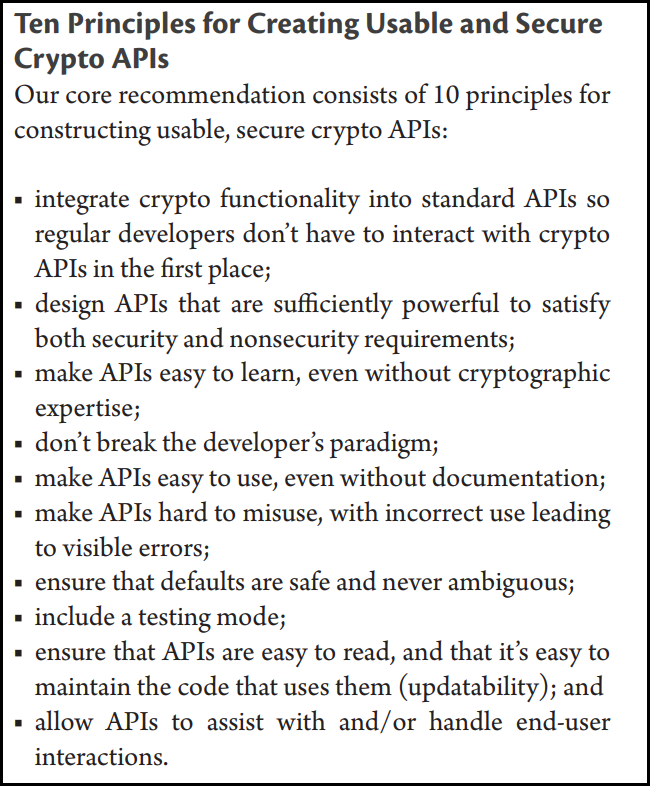
\includegraphics[width=0.65\textwidth]{GreenPrinciples}
\caption{10 Design Principles for Cryptography APIs by Green \& Smith (2016, \cite{green2016}, p. 42)}
\label{fig:Princip}
\end{figure}

\par
Patnaik \etal extended these principles by defining usability smells \cite{patnaik2019}.
They were looking for "telltale signs, that one of the ten usability principles is being violated" (2019, \cite{patnaik2019}, p. 245).
They examined a wide range of popular cryptography APIs: OpenSSL, NaCl, libsodium, Bouncy Castle, SJCL, Crypto-JS, and PyCrypto.
They manually reviewed almost 2500 posts on Stack Overflow and tried to identify the issues the programmers were facing.
They identified 16 thematic issues of which 2 related to the programmers' lack of knowledge:
\begin{itemize}
	\item \emph{Passing the buck}: Questions that are answered in the documentation
	\item \emph{Lack of Knowledge}: Questions implying that "the developer does not have foundation level cryptography knowledge" (Patnaik \etal, 2019, \cite{patnaik2019}, p. 250).
\end{itemize}
They mapped the remaining issues to four usability smells:\\
\begin{figure}[h]
\centering
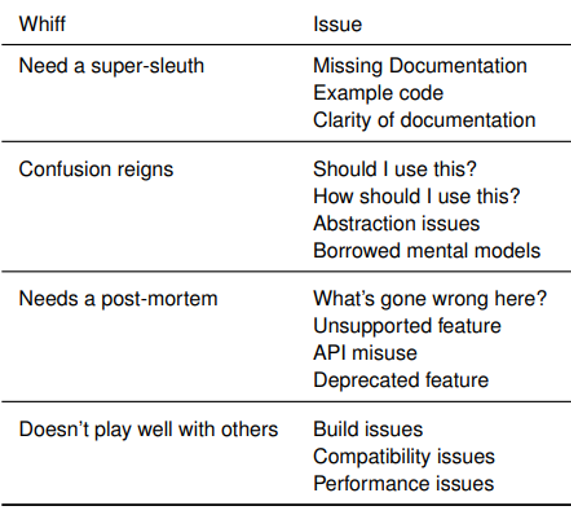
\includegraphics[width=0.6\textwidth]{UsabilitySmells}
\caption{Usability Smells and Issues as defined by Patnaik \etal (2019, \cite{patnaik2019}, p. 254)}
\label{fig:Smells}
\end{figure}

\par
Hazhirpasand \etal selected 20 popular cryptography libraries and
evaluated 25 Stack Overflow posts for each one of them \cite{hazhirpasand2021_b}. 
They assigned a topic to each one of them (see figure \ref{fig:topic}).
\begin{figure}[h]
\centering
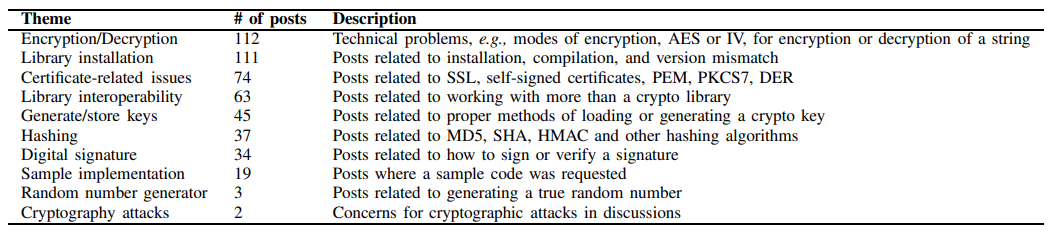
\includegraphics[width=1\textwidth]{topics}
\caption{Topics Discussed on Stack Overflow Regarding Cryptography Libraries (Hazhirpasand \etal, 2019, \cite{hazhirpasand2021_b}, p. 4)}
\label{fig:topic}
\end{figure}
They found that the prevalence of topics differs between the libraries.
As an example, users of pyOpenSSL mainly struggled with certificates (17), mcrypt users had difficulties installing the library (16),
and more than half of the posts referring to CryptoJS library were about library interoperability (13).
Yet, many cryptography libraries share the same problems.\\
\newpage
\par
Acar \etal evaluated and compared five cryptography libraries for python \cite{acar2017}.\footnote{cryptography.io, Keyczar, PyNaCl, M2Crypto, and PyCrypto}
Their aim was to understand the reasons for failure (or success) when implementing cryptography scenarios and to define a blueprint for a new, more usable cryptography libraries.
They conducted a between-subjects online study where python programmers had to implement a symmetric or asymmetric encryption task using an assigned library.
Both, task and library, were assigned randomly.
The programmers also had to fill out an exit survey where they were asked about their backgrounds as well as their opinion regarding the assigned task and library.
Acar \etal then examined the submitted code regarding functionality and security and controlled their findings for the participant's background.\\
They found that the strongest predictors for working code was the documentation quality and the availability of working code examples.
When it comes to security, the programmers background was most important. Developers with a security background were more likely to produce secure code.
Although "simpler" APIs\footnote{more abstract, secure default values} seemed to promote better security results, they did not completely solve security problems.
The key issues regarding security were that libraries did not support auxiliary tasks (\ie key storage) and lacking documentation quality.
Acar \etal also observed that a complex API with good documentation (\ie PyCrypto) was rated more usable by the participants than a simple API with bad documentation (\ie Keyczar).\\

\par
Mindermann \etal evaluated the usability of Rust cryptography libraries \cite{mindermann2018}.
After determining the most popular libraries, they conducted an exploratory study where one of the authors completed a set of cryptography related task several times using a different library for each round.
They afterwards compared two popular libraries, rust-crypto and ring, in a controlled experiment.
Students had to complete a code skeleton by adding symmetric encryption logic.\\
They found that the older "low-level" but more powerful libraries (\ie rust-openssl, rust-crypto) lacked usability whereas others made a great effort to provide it (\ie rust-sodium, sodiumoxide). 
Similarly, high-level libraries use authenticated encryption by default, whereas Mindermann \etal considered that this was not advertised enough in low-level libraries.
Default values were often avoided, but if present, they were secure.
Yet, there were some security risks:
Some libraries did not warn about broken algorithms or did not give any warnings when a nonce was accidentally reused.
Documentation quality varied between and within the libraries.\\
Mindermann \etal also issued 12 recommendations to remedy present usability issues.
These were more specific than the ones by Green \& Smith as they only applied to Rust libraries.\\

\par
Nadi \etal investigated the usability of Java cryptography libraries.
They wanted to understand the underlying causes for misuse of the related APIs.
They also aimed to identify the most common cryptography tasks and possible support tools.\\
Nadi \etal followed several approaches:
They manually reviewed 100 posts on Stack Overflow, examined 100 GitHub repositories and conducted two surveys.
Regarding the usability of Java cryptography libraries, they found that the biggest obstacles were the lack of documentation (\ie code examples), the APIs' design (\ie error messages, method overloading, insecure default values), and lack of domain knowledge among programmers.
The participants of the surveys explicitly asked for more abstract APIs and better documentation.\\





% API Misuse
\section{Misuse of Cryptography APIs}
Krüger \etal proposed CrySL, a definition language that allows to specify rules for secure usage of cryptography API \cite{kruger2017}.
It allows to specify rule sets classwise in separate files. Krüger \etal also implemented CogniCrypt, a compiler that translates CrySL rules into a static analysis that automatically checks a given Java application for rule violations \cite{kruger2017}.\\
To evaluate it, they defined  a rule set for JCA library and analyzed 10,001 Android apps.
They also reviewed 50 Apps manually for comparison.
CogniCrypt detected the use of JCA in 4,071 apps.
In 96 \% of them, CogniCrypt identified at least one issue.
In total, CogniCrypt discovered 19,756 rule violations.
Most of them referred to broken constraints (\ie illegal values), especially for the \lstinline|MessageDigest| class.
In the manual analysis, Krüger \etal found that some programmers still used MD-5 and SHA-1 hash functions although these are considered broken.
CogniCrypt also identified a large number of misuses of the \lstinline|Cipher| class, especially the use of broken algorithms (\ie DES) and unsafe encryption modes (\ie ECB).
Another common misuse was that programmers forgot to clear the password at the end of the lifetime of a \lstinline|PBEKeySpec| object.\\

\par
Hazhirpasand \etal also used CogniCrypt to analyze 489 open source Java projects that made use of the JCA library \cite{hazhirpasand2020}.
Only 2 of them were considered as completely secure.
\begin{figure}[h]
\centering
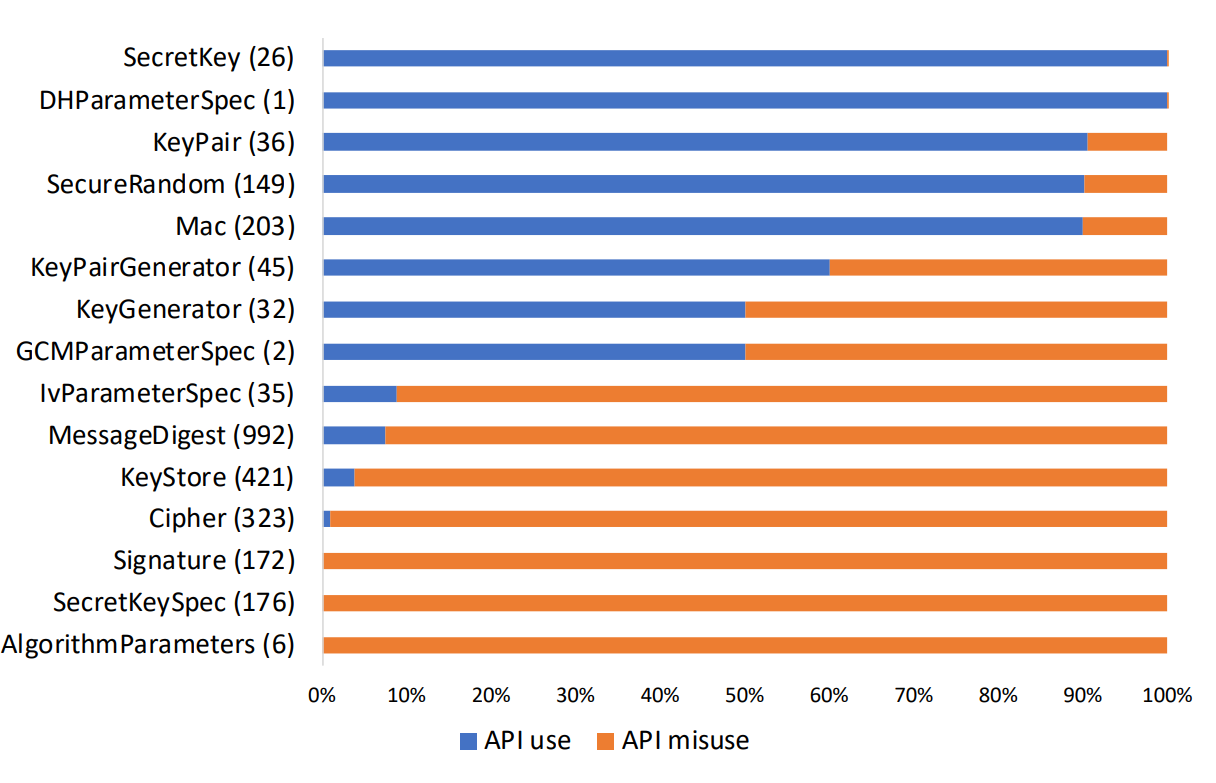
\includegraphics[width=0.9\textwidth]{APIMisuse}
\caption{Correct API use vs. API Misuse (Hazhirpasand \etal, 2020, \cite{hazhirpasand2020}, p. 3)}
\label{fig:APIMisuse}
\end{figure}
Figure \ref{fig:APIMisuse} shows the ratio of correct and incorrect usage for each of the investigated APIs.
Although a few records were mistakenly marked as misuse according to the authors manual review, their findings showed that programmers especially struggled to use the classes
\lstinline|AlgorithmParmeters|, \lstinline|SecretKeySpec|, \lstinline|Signature|, \lstinline|Cipher|,\lstinline|KeyStore|, \lstinline|MessageDigest|, and \lstinline|IVParameterSpec| correctly.
These classes support (symmetric) encryption, hashing, and digital signatures.\\
Hazhirpasand \etal also contacted 216 maintainers of the repositories to understand the reasons for API misuse.
Their answers implied that developers often underestimated the impact of cryptography misuse in publicly accessible code. 
They were not aware that 
and were not aware that their publicly accessible code could influence other programmers who were looking for examples. 
Some maintainers also lacked security knowledge.
They did not know how to use the API correctly and accepted security related pull request blindly.
Another identified issue was that there were not enough security concerns in the official documentation.
Sometimes, programmers also argued that although they use a cryptographic API, the code was not security related.\\

\newpage
\par
Piccolboni \etal also developed a tool to check security related code for API misuse: CRYLOGGER \cite{piccolboni2020}.
It conducts a dynamic analysis by logging the parameters that are passed to the cryptography APIs during the execution.
It later checks their legitimacy using a list of security related rules (see figure \ref{fig:CryloggerRules}).
\begin{figure}[h]
\centering
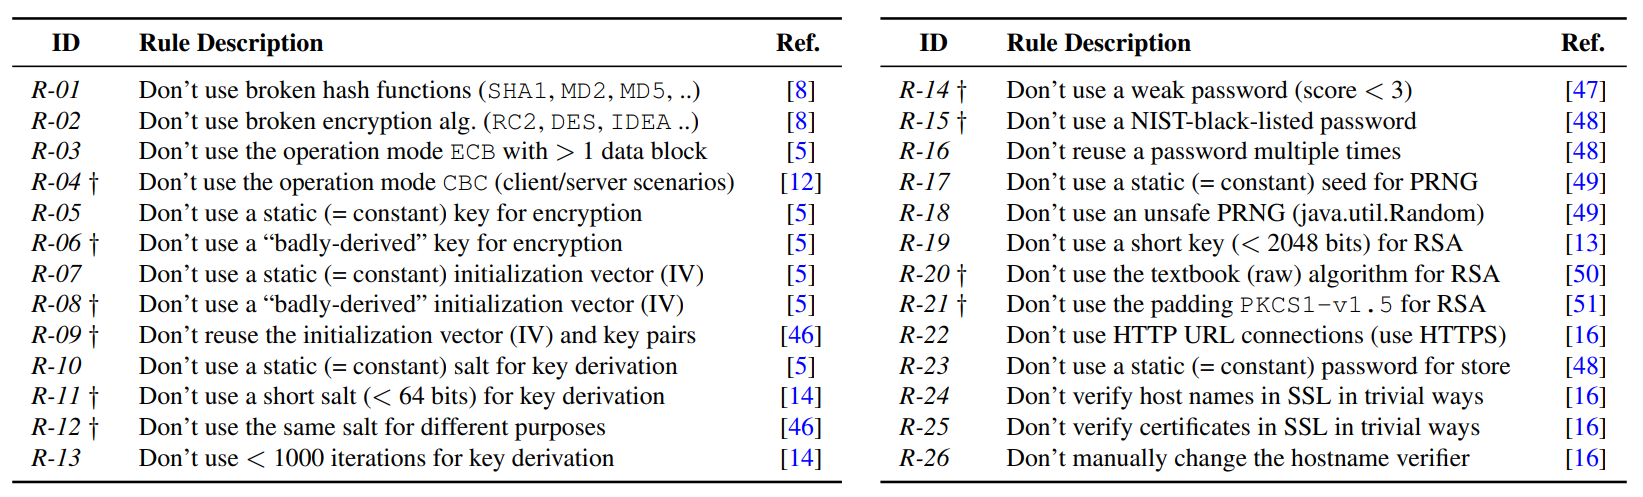
\includegraphics[width=1\textwidth]{CryloggerRules}
\caption{CRYLOGGER's Security Rules (Piccolboni \etal, 2020, \cite{piccolboni2020}, p. 5)}
\label{fig:CryloggerRules}
\end{figure}
Piccolboni \etal used CRYLOGGER to analyze 1,780 Android apps.
They found that rules 01 and 18 were violated very often ($> 90\%$).
This implied that broken hash functions and unsafe sources for random number generation were used frequently.
They also found a rather high prevalence of violations for rules 04, 05, 06, 07, 09 and 22 ($> 30\%$) which refer to unsafe keys and initialization vectors (IVs), the reuse of key-IV pairs and the use of HTTP protocol.\\
\begin{figure}[h]
\centering
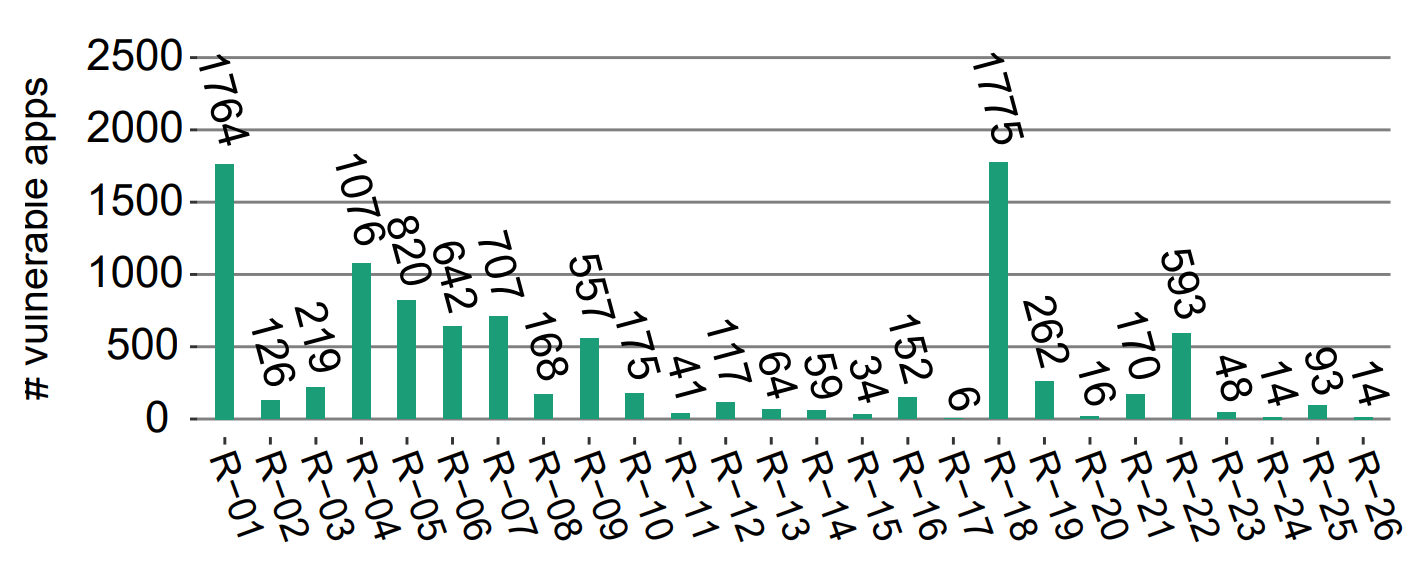
\includegraphics[width=0.7\textwidth]{RVPiccolboni}
\caption{Rule Violations Detected by CRYLOGGER ($N=1,780$) (Piccolboni \etal, 2020, \cite{piccolboni2020}, p. 12)}
\label{fig:CryloggerRules}
\end{figure}
\\
\par
Hazhirpasand \& Ghafari \cite{hazhirpasand2021_a} followed a different approach and analyzed 173 vulnerability
reports on the HackerOne bug bounty platform to understand
the existing types of cryptography vulnerabilities.
Most of them (33.5\%) referred to the use of insecure SSL versions.
Other common topics were the use of weak cryptography parameters (\ie broken hashing algorithms, short keys) (14.5\%), OpenSSL bugs (14.5\%), and mixing HTTP/HTTPS content (12.7\%).
In rarer cases, the reports were about miscellaneous attacks (6.9\%), timing attacks (6.3\%), the use of static keys or passwords (6,3\%), or issues related  to HTTP (5.2\%).



% === M E T H O D O L O G Y ===
\chapter {Methodology}
\label{cha:Method}
To answer our first research question\footnote{What issues do programmers face when implementing symmetric encryption using Java Cryptography Architecture?}, we had to identify the issues programmers face when implementing symmetric encryption using JCA.
We derived such issues by analyzing 150 threads on Stack Overflow, which is one of the most popular Q\&A forums for programmers.
To answer our second research question\footnote{What are common security risks in code and advice shared on Stack Overflow referring to the implementation of symmetric encryption scenarios using JCA library?}, we also scanned these threads regarding security risks.
Based on the elicited issues, we then attempted to define a set of questions in order to observe to what extent for these questions the official documentation provides us with answers.
This helped us answering the third research question.\footnote{To what extent are these issues linked to missing or inadequate documentation?}\\

\par
As we required several methodical approaches, this chapter is divided into five sections.
The first section describes the sampling process.
The second section refers to identifying issues from Stack Overflow posts.
The third section explains how we checked the threads for security issues.
The fourth section is about deriving questions from the previous findings and analyzing of the library's documentation.
The fifth section illustrates the evaluation processes.\\

\newpage
% === Sampling ===
\section{Sampling}
\label{cha:MetSampling}
In Java, developers should use the \lstinline|Cipher| class in order to accomplish a symmetric encryption task.
The class supports a wide range of symmetric and asymmetric encryption algorithms.
To search for suitable threads on Stack Overflow, we first defined a set of queries.
We use the \lstinline|[java]| tag combined with a minimal \lstinline|Cipher.getInstance()| statement for each symmetric algorithm.
This statement must be executed in all encryption scenarios using the \lstinline|Cipher| class.\\
As some of the symmetric algorithms supported by JCA are not very popular, the corresponding queries returned only a small amount of posts.
We decided to exclude these algorithms, such as RC2, and focused on the three most popular symmetric encryption algorithms: AES, 3DES\footnote{also TripleDES, DESede} and DES.
We therefore used three queries which are shown in the left column of table \ref{tab:SampleSize}.\\
\par
Next, we calculated the sampling size using the \href{https://www.surveymonkey.com/mp/sample-size-calculator/}{sample size calculator by SurveyMonkey}.
To ensure a confidence level of 95\% and a margin of error below 8\%, we needed to study 150 posts.
Then, we computed sample size per each query proportionally to the number of posts a it returned.
The result can be found in table \ref{tab:SampleSize}.
\begin{table}[h]
\centering
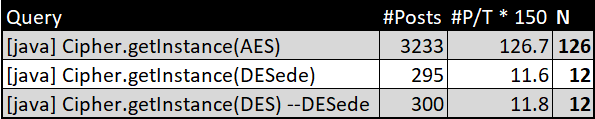
\includegraphics[width=0.7\textwidth]{SampleSize}
\caption{Computation of Sample Sizes}
\label{tab:SampleSize}
\end{table}

\par
Finally, to select the threads from Stack Overflow, 
we chose 50\% of the sample size from the newest threads and the other half from the most popular ones.
Using this approach, we attempted to balance the inclination of our sample size since the majority of developers first look for answers on Stack Overflow before posting a question.\\
As the aim of the analysis was to reveal issues referring to the implementation of \emph{symmetric encryption} using the \emph{JCA} library, we excluded all posts that did not refer to this scope.
A complete list of reasons for exclusion and some example threads is available in the appendix.
However, a thread commonly consists of more than one issue.
Therefore, we included the threads in which at least one issue, question, or advice was referred to our scope.
As we also did not include any posts of lacking quality, 
we had to exclude 296 threads.

\newpage
% === Analysis 1 ===
\section{Analysis of Issues}
\label{cha:MetIssues}
The goal of the first analysis was to answer the first research question: \emph{What issues do programmers face when implementing symmetric encryption using Java Cryptography Architecture?}
We conducted a manual qualitative content analysis following the guidelines by Mayring \cite{mayring2015}.
As our sample is rather large to analyse it qualitatively by hand, we needed an approach that allowed to evaluate large amount of data efficiently. Also, we needed it to support method-integrative approaches that combine qualitative and quantitative elements.
These are the key characteristics of Mayring's guidelines.
They also provide a set of criteria to evaluate the validity and reliability of a methodical approach.\\
In this section, we will only provide the information to understand the process. You can find the complete processing scheme in the "Anleitung zu Wissenschaftlichen Arbeiten", chapter \ref{cha:AWI}.\\
\par
We conducted the analysis in three rounds.
We first applied \emph{summarizing} to extract the relevant information (issues and questions) from the threads.
Then we classified the issues in two rounds.\\

% === Summarizing ===
\subsection{Summarizing}
In this step, the goal was to extract and record all relevant information such that we did not have to re-read the entire threads during the further evaluation steps.
In our analysis, we considered the question post, posts marked as "accepted answers" as well as comments.
If there was not an accepted answer in a thread, we considered all posts and comments.\\
There were two coders involved in summarizing.
We conducted summarizing first independently and then discussed the results with each other to create a consistent and more objective list of records.
In particular, we eliminated records that did not refer to our scope.
As an example, we excluded all issues that referred to the conversion of plain text or cipher text (\ie character encoding).\\
\par
For each thread, we recorded the set of issues and questions that the original poster\footnote{author of the question post} was facing.
Sometimes, we also identified issues based on comments, \ie security hints.
Then we tried to identify the reasons and solutions from the accepted answer post.
If no answer was accepted, we tried to derive it from the discussion, \ie based on a comment by the original poster indicating that a comment was helpful.\footnote{Comments cannot be marked as accepted answer}
If there was not any indication on what advice was helpful, we recorded all advice and recommendations from the discussion.
Sometimes, we were also not able to find any possible explanations for the original poster's issues.\\
As a result, we aimed for one record per issue that must consist of a short description\footnote{\ie an error message, a shortened form of a question} and might include more precise explanations for the reason the solution.

% === Classification ===
\subsection{Classification}
All records that resulted from summarizing were classified in two rounds:
First, we categorized all records regarding technical aspects and second, regarding requirements the original poster was not able to meet.
Per round, we assigned at most one category to each record.\\

% Technical Aspects / Implementation
\subsubsection*{Technical Aspects}
In the first round of classification, we focused on the technical aspects of implementing symmetric encryption.
We focused on the issues that prevented the original posters from producing code that compiled and ran without throwing an error.
We started with a set of predefined main categories which we inductively refined during the classification.
Each time we defined a new category, we restarted the classification.\\

\par
The main categories referred to the set of tasks that programmers must take care of when implementing symmetric encryption using JCA:
\emph{Cipher Object Instantiation, Generating Algorithm Parameters, Cipher Object Initialization, Transformation, and Transmitting Algorithm Parameters}.
We defined subcategories to get deeper insight (\ie if a issue targeted only one aspect of a main task), or to allow unambiguous classification (\ie dependencies between two properties). 
We also added one more main category.
We ended up with the following \textit{main} and \textbf{subcategories}:
\begin{itemize}
	\item \textit{Cipher Object Instantiation}:
				We assigned this category to all issues and questions referring to an inappropriate \lstinline|Cipher.getInstance(...)| statement.
				As parameter, programmers must pass a transformation string consisting of:
				\begin{itemize}
					\item \textbf{Algorithm} (mandatory)
					\item \textbf{Encryption Mode} (optional)
					\item \textbf{Padding Mode} (optional)
				\end{itemize}
				Additionally, we defined the following subcategories:
				\begin{itemize}
					\item \textbf{Dependency Encryption Mode - Padding}: The encryption modes determines whether padding is required or not.
								We assigned this category to all issues caused by an inappropriate specification of these two properties.
					\item \textbf{Cipher Object Instantiation - Other} for issues and questions related to \lstinline|Cipher| object instantiation but not any of the aforementioned aspects.
				\end{itemize}
	\item \textit{Generating Algorithm Parameters}: 
				Depending on the specification of the cipher object, it requires different kind of parameters. 
				For encryption, the programmer might need to perform the following tasks:
				\begin{itemize}
					\item \textbf{Key Derivation} for issues and questions referring to random key generation, password based key derivation or key exchange protocols.
					\item \textbf{Initialization Vector / Nonce Generation} for issues and questions referring to the generation of the IV or nonce used for the transformation.
					\item \textbf{Generation of Other Algorithm Parameters}, e.g. a \lstinline|GCMParameterSpec| object which contains additional parameters for GCM encryption mode.
				\end{itemize}
	\item \textit{Cipher Object Initialization}: We assigned this category to all issues caused by the misuse of the \lstinline|init(...)| statement, e.g. not passing all required
						parameters. We defined the following subcategories:
				\begin{itemize}
					\item \textbf{Dependency Algorithm - Key}: The algorithm determines what data type the key must be stored in. 
									It also defines the allowed key sizes.
									We assigned this category to issues caused by passing an inappropriate key to the \lstinline|init(...)| method or questions about this dependency.
					\item \textbf{Dependency Algorithm \& Encryption Mode - IV}: The encryption mode determines, whether an IV is required or not.
									For some encryption modes (e.g. "CBC") the IV must be the same size as the algorithms block size.
									As an example, an issue related to passing an IV of the wrong size to the \lstinline|init(...)| method was assigned to this category.
					\item \textbf{Cipher Object Initialization - Other}
				\end{itemize}
	\item \textit{Transformation}: This category was assigned to all issues and questions targeting the actual transformation methods \lstinline|update(...)| and \lstinline|doFinal(...)|, e.g. passing the wrong input parameters or questions about the output.
	\item \textit{Transmission of Parameters}:
				As all parameters from encryption must be reused for decryption, they must either be stored or transmitted. 
				This category was assigned to all issues and questions referring to storing, restoring, or transmitting parameters.
				We defined the following subcategories:
				\begin{itemize}
					\item \textbf{Key Transmission}: The key must be kept secret.
					\item \textbf{Transmission of Other Parameters} such as the initialization vector. 
						They can be transmitted along the cipher text as they do not have to remain secret.
	 			\end{itemize}
	\item \textit{Dependency Encryptor - Decryptor}: 
				The \lstinline|Cipher| objects used for encryption and decryption must be specified and initiated in the exact same way except for the parameter specifying the operation in the \lstinline|init(...)| statement.
				We assigned this category to all issues caused by differing configurations.
\end{itemize}

\begin{figure}[h]
\centering
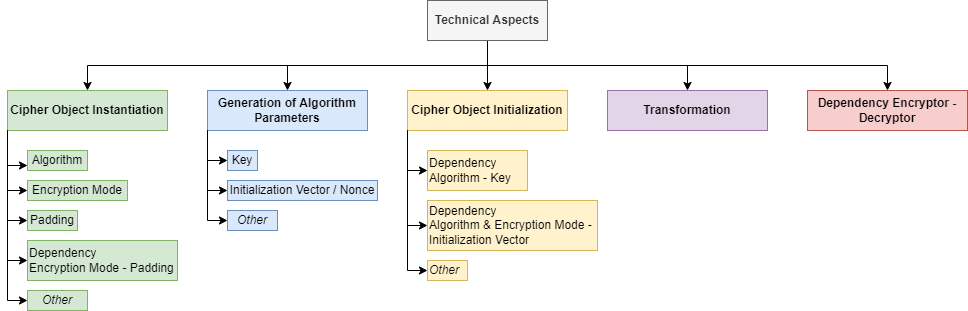
\includegraphics[width=1\textwidth]{Categories}
\caption{Hierarchy of Technical Aspects Categories}
\label{fig:Categories}
\end{figure}

\par
If all tasks are implemented correctly, the code compiles and runs without raising any error.
Therefore, if programmers ask questions on Stack Overflow about a technical aspect, they either implemented a task incorrectly or they have a question regarding one of these tasks.
During this first classification round we asked 
"What implementation step was performed incorrectly causing the error?" or 
"What implementation step is targeted by the question?".\\



% Implications / Requirements
\subsubsection*{Requirements}
Unlike the first set of categories targeting the implementation of symmetric encryption, we defined a second set of categories regarding the design of an application.
We defined different kinds of functional and non-functional requirements as categories.
We consulted  Sommerville \cite{sommerville2011} as a theoretical basis.
During the analysis we asked ourselves "Which requirements are not met?".
Not all requirements defined by Sommerville occurred in our analysis and therefore, we only assigned the following categories:
\begin{itemize}
	\item \textbf{Use Case} to issues where a programmer was not able to fulfill a certain functional requirement or tried to use encryption for an unsuitable use case.
	\item \textbf{Performance} to issues where an implementation was not as time-efficient as required.
	\item \textbf{Space} to code leading to an \lstinline|OutOfMemoryException|.
	\item \textbf{Reliability} to situations where the implementation crashed frequently.
	\item \textbf{Portability} to implementations that behaved differently on different (Java) platforms.
	\item \textbf{Interoperability} to issues where a developer was not able to decrypt a cipher text that was produced using another library or vice versa.
	\item \textbf{Security} to implementations containing security risks.
\end{itemize}
\par
As we analyzed the discussion, we only assigned a category if either the original poster complained about not being able to meet a certain requirement or someone warned that the shared code might cause issues regarding one of the requirements (\ie a security hint).\\
\par
A list of examples for each category is available in the appendix.



% === Analysis 2 ===
\section{Analysis of Security Risks}
\label{cha:MetSec}
The goal of second analysis was to answer the second research question: 
\emph{What are common security risks in code and advice shared on Stack Overflow referring to the implementation of symmetric encryption scenarios Java Cryptography Architecture?}\\
We first defined a set of security rules regarding the implementation of symmetric encryption.
Then we manually checked the threads from our sample for violations of these rules.

\subsection{Security Rules}
We derived our rules from the rule sets used for CRYLOGGER tool (Piccolboni \etal \cite{piccolboni2020}) and CogniCrypt (Krüger \etal \cite{kruger2019}).
We only considered the rules that were applicable to symmetric encryption and structured them using the categories from technical aspect's classification (see section \ref{cha:MetIssues}).
We also generalized them to simplify the evaluation.
As an example, R-04 of CRYLOGGER says " Don’t use the operation mode CBC (client/server scenarios)" (Piccolboni \etal, 2020, \cite{piccolboni2020}, p.5).
As we often did not know in what context the original poster wanted to use the code, we defined that CBC should not be used at all.
The resulting rules can be found in table \ref{tab:Rules}.
\begin{table}[h]
\centering
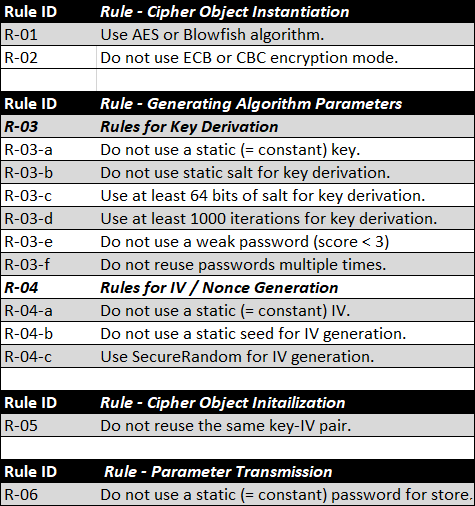
\includegraphics[width=0.7\textwidth]{Rules}
\caption{Security Rules}
\label{tab:Rules}
\end{table}

\subsection{Tracking Security Rule Violations}
We manually checked the original sample in order to observe any security rule violation.
We only considered the question post, the accepted answer post, and comments to one of these.
We also distinguished between "question" and "answer" as well as "code" and "text".
We analyzed the four aspects independently and made a list for each one of them:
\begin{itemize}
	\item \textbf{Question Code} to track security risks in code snippets of the question post
 	\item \textbf{Question Text} to track security risks in the text of the question post as well as comments to it by the original poster
	\item \textbf{Answer Code} to track security risks in code snippets of the answer post
	\item \textbf{Answer Text} to track security risks in the text of the answer post as well as any comment by another person.
\end{itemize}
While analyzing the code snippets, we focused on the parts where encryption, decryption, key derivation, IV generation, and key storage were implemented.
As an example, if someone defined a key in the main method and passed it to the encryption section as a parameter, we did not consider this a security risk.
The encryption section can still be safe if an appropriately derived, non-static key is passed.\\


% === Analysis 3: Documentation ===
\section{Analysis of Documentation}
\label{cha:MetDoc}
The results from the preceding analyses formed the basis to analyze the documentation for JCA.
As it spreads over several documents and sources, we only examined the most basic ones:
the Java Cryptography Architecture (JCA) Reference Guide \cite{javaReferenceGuide}, 
the Java Security Standard Algorithm Name Specification \cite{javaStandardAlgorithmName}, 
and the entire API documentation for \lstinline|javax.crypto| package starting from the package overview \cite{javaxCrypto}.
These three documents are valid for all providers and therefore apply to a wide range of platforms.\\
\par
To analyze the documentation, we first defined a set of question that should be answered.
Afterwards, we sought the answers in the documentation.
Our aim was to answer the third research question: 
\emph{To what extent are these issues linked to missing or inadequate documentation?}
The questions additionally gave us more insight into what programmers are struggling with (first research question).

\subsection{Deriving Questions}
Generally speaking, the official documentation should support the usage of the API and not educate developers or their basic questions regarding cryptography.
However, the documentatin of a cryptographic API should link reliable and comprehensible resources that explain basic cryptographic concepts (Mindermann \etal \cite{mindermann2018}).
We therefore created two lists of prioritized questions: one with "questions for documentation" and one containing "general questions".\\
\par
We derived the questions from the results of the first analysis.
We reprocessed the records and tried to formulate a question for each one.
If the question was new, we wrote it down and set its priority to one.
If there was already a similar question, we increased its priority by one and sometimes reformulated the question.\\
Then, we adapted the priorities of the questions referring to security based on the results of the second analysis.
We set the priority to the actual number of posts targeted by it.

\subsection{Consulting Documentation}
For each question on the list, we then tried to find an answer in the documentation.
Depending on the question, we checked the resources in another order.
We aimed to find answers as time-efficiently as possible.\\
For "questions for documentation", we typically started with the reference guide to find general explanations and then consulted the related parts of the API documentation.
For "general questions" we started in the standard algorithm name specification.
Of course, we knew the documentation better after answering a set of questions and therefore optimized our search strategies.\\
Once we found an answer to the question, we recorded its source as well as some remarks regarding documentation quality (see section \ref{cha:DocQuality}).

\section{Evaluation}
\label{cha:MetEva}
After the first analysis (section \ref{cha:MetIssues}), we applied several forms of frequency analysis to identify the tasks and requirements most programmers were struggling with.
We similarly evaluated the results from the second analysis (section \ref{cha:MetSec}) to identify the most common security risks.\\
After the third analysis (section \ref{cha:MetDoc}), we interpreted the results in several ways.
We had a closer look at the questions' content as well as their priorities.
Also we wanted to know how many and what questions were answered by documentation.
We tried to identify possible relations between issues and security risks on one side and documentation (and API design) on the other side.
Finally, we made recommendations on how the documentation of JCA could be improved.




% === R E S U L T S ===
\chapter {Results and Interpretations}
\label{cha:Results}
In this chapter, we discuss the results of our three analyses and their interpretation.
There is a section for each of the three conducted analyses:
The first section presents the issues programmers faced during the implementation of a symmetric encryption scenario using JCA library.
The second section discusses the security risks we found in our sample data.
The third section explains how the previous findings are linked to the documentation.\\


% === Issues ===
\section{Implementation Issues}
\label{cha:ResIss}
In our first analysis, we tried to identify all issues the original posters were facing and recorded them separately.
Depending on what the original poster was struggling with, we afterwards classified the issues as relating to a \emph{technical aspect} and/or a \emph{requirement}.\\
In total, we recorded 219 issues.
We classified 197 (90\%) of these records regarding technical aspects and 76 (35\%) regarding requirements. 
62 records were classified twice.
We could not classify only one thread (and its relating record) to the lack of adequate information.\\
\begin{figure}[h]
\centering
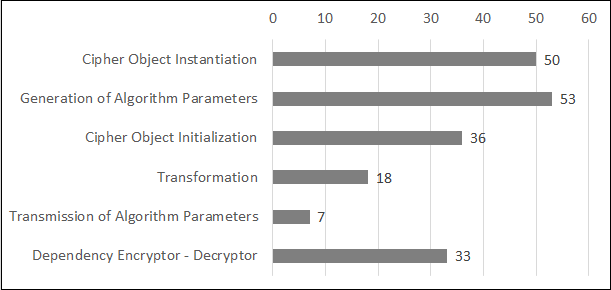
\includegraphics[width=0.85\textwidth]{TechnicalAspects}
\caption{Number of Issues Assigned to a Technical Aspects Main Category ($N = 219$)}
\label{fig:TechAspPlot}
\end{figure}

\par
% === Technical Aspects ===
As shown in figure \ref{fig:TechAspPlot}, the most common categories in the first round of categorization were \emph{Generation of Algorithm Parameters} (50) and \emph{Cipher Object Instantiation} (53). 
Both of these categories refer to specifying and generating the properties that are used during encryption or decryption.
During the generation of algorithm parameters, programmers might derive a key, an initialization vector, and other algorithm parameters such as advanced authentication data.
The original posters especially struggled with key derivation (36 records - 16.4\%).
This was not surprising as previous work has already revealed that programmers struggled with key handling.
The set of issues referring to the key\footnote{derivation, transmission, dependency from algorithm} made up more than $\frac{1}{5}$ of all issues.\\
During the instantiation of a \lstinline|Cipher| object, programmers specify the algorithm, the encryption mode, and padding.
The original posters were especially struggling with the latter two.
18 records referred to the encryption mode, 11 to padding and another 11 to the dependency of these properties\\
\par
The third most common category was \emph{Cipher Object Initialization} (36). 
In this implementation step, the generated parameters (\ie key, IV,...) are passed to the cipher object.
Most issues were assigned to the \emph{other} subcategory.
They often refer to the original posters not passing all required parameters of the \lstinline|init(...)|.\\
The fourth most common category was \emph{Dependency Encryptor - Decryptor} (33).
More than 27\% of all issues referred to a dependency related subcategory.
The high prevalence of issues referring to the dependency of encryptor and decryptor implies that people lack knowledge about (symmetric) encryption in general.\\
The fact that the cipher objects for encryption and decryption must use the exact same algorithms and parameters is \emph{the} basic principle of symmetric encryption.\\

\par
The other main categories and subcategories were not assigned that often.
Some original posters were confused that there were 2 methods that perform \emph{Transformation}: \lstinline|update(...)| and \lstinline|doFinal(...)|.
They did not know which method must be called in their scenario.\\
Among issues referring to the \emph{Transmission of Algorithm Parameters} (7), most referred to the key (5).
The remaining records were related to the initialization vector (1) and the salt used for password based key derivation (1).\\
\par
You can find the complete list of subcategories and their frequencies of assignment in table \ref{tab:TechAspTab}.\\
\begin{table}[h]
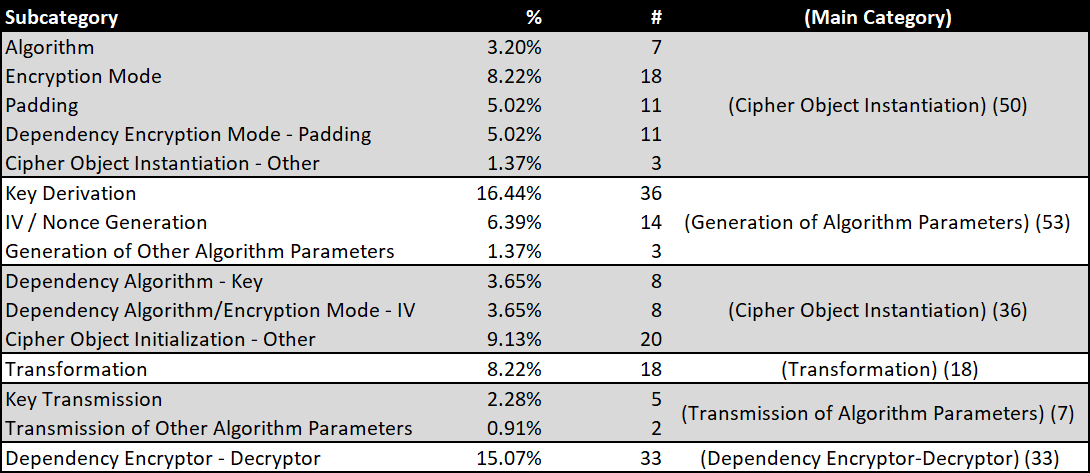
\includegraphics[width=1\textwidth]{TechAspTable}
\caption{Number of Issues Assigned to a Technical Aspect Subcategory ($N = 219$)}
\label{tab:TechAspTab}
\end{table}

% === Requirements ===
\par
Within the categories referring to requirements, \emph{Security} was the dominating category (46 records - 21\%).
This seems natural as this is what cryptography is all about.
However, only 3 original posters asked about the security of their implementation.
One person asked whether the IV used by default is safe.
Another person asked whether it was secure to reuse algorithm parameters (\ie key, IV) for several transformations.
The third person asked whether encryption got safer if some kind of salt was added to the plain text.
A more common security issue was that programmers were not able to run AES-256 due to missing security policy files (5 threads).
However, most security records were identified based on security hints from people commenting or answering the questions.
Yet, there is massive under-reporting as our results from the security related analysis show (see section \ref{cha:ResSec}).\\
\begin{figure}[h]
\centering
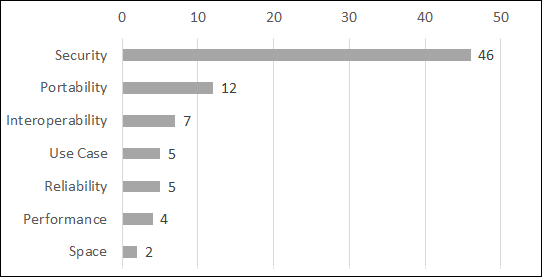
\includegraphics[width=0.8\textwidth]{Requirements}
\caption{Number of Issues Assigned to a Requirement Category ($N = 219$)}
\label{fig:Req}
\end{figure}
\par
As shown in figure \ref{fig:Req}, the other requirement categories occurred less often.
There were 12 issues related to the \emph{Portability} of an application.
They often refer to original posters not specifying all values themselves.
As an example, several programmers only passed "AES" to the \lstinline|Cipher.getInstance(...)| method.
In that case, default values are used for encryption mode and padding.
These values however differ between different providers and therefore between different platforms.\\
Another 7 records were assigned to \emph{Interoperability} category.
These issues occurred if original posters implemented one task in different ways in both source codes.
Sometimes, the other library was more abstract and used default values (\ie for padding) that were therefore not visible in the source code.
As a result, the original posters instantiated or initialized the Java \lstinline|Cipher| objects incorrectly.
Some of these default values were also not supported by JCA (\ie ZeroPadding).
Some programmers also used non-standardized functions (\ie SHA1PRNG for random number generation).\\
The 5 issues referring to \emph{Use Case} category related to the misuse of encryption for an inappropriate use case (2), to a use case that was not supported by JCA library (2) and a use case that is just not possible to implement (1, mapping 16 B of data bijectively to a 12 digit number).\\
Most of the issues that were assigned to the \emph{Reliability} category were caused by the original poster declaring \lstinline|Cipher| objects statically in global space.
The application crashed frequently because \lstinline|Cipher| objects are not thread-safe.\\
Some programmers complained that the execution of \lstinline|getInstance(...)| method was taking too long (lacking \emph{Performance}).
One original poster also observed that the encryption of a large file was time consuming.
Other developers reported that an \lstinline|OutOfMemoryException| occurred when they tried to encrypt a large file at once (lacking \emph{Space} efficiency).\\

\par
% === Doubly Classified Records ===
As previously mentioned, some records were classified twice, regarding technical aspects and requirements.
The heat map in figure \ref{fig:HeatMap} shows the relative overlapping of categories.
We observed the highest overlapping of categories for \emph{Generation of Algorithm Parameters} and \emph{Security}.
21\% of all records assigned to \emph{Generation of Algorithm Parameters} or \emph{Security} category were assigned to both categories.
Most of them referred to static values being used for key or initialization vectors.
The second highest overlapping was between \emph{Cipher Object Instantiation} and \emph{Security} categories (16\%). 
Almost all of them referred to the use of an unsafe encryption mode.\\
As we had less data for the other requirements categories, it is not surprising that we found much less overlapping for these.
The issues that were assigned to the \emph{Portability} or \emph{Interoperability} category and some other technical aspects category were mostly due to default values that vary between platforms and libraries.
The overlapping with \emph{Reliability} category indicated where the applications crashed: during \emph{Cipher Object Initialization} or \emph{Transformation}.
The bi-classification of \emph{Cipher Object Instantiation} and \emph{Performance} implied that the execution of this function is particularly time consuming.

\begin{figure}[h]
\centering
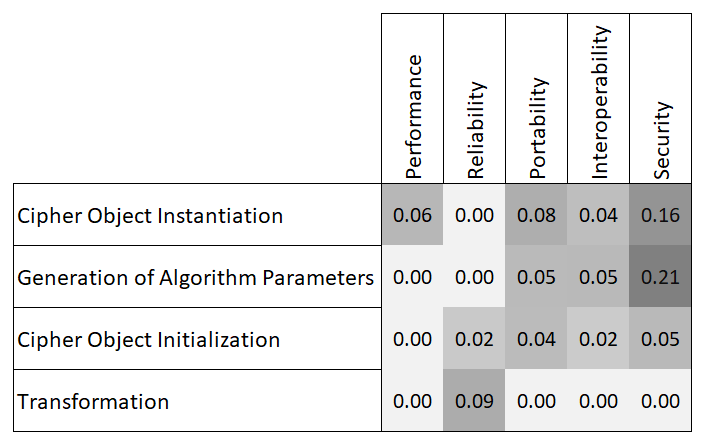
\includegraphics[width=0.8\textwidth]{HeatMap}
\caption{Relative Overlapping of Technical Aspects and Requirements Categories}
\label{fig:HeatMap}
\end{figure}



\newpage
% === Security ===
\section{Security Risks}
\label{cha:ResSec}
We manually checked 150 question,  84 answer posts, and related comments to find any violations against our rule set.
We found a total of 331 security risks.
Most of them (249 - 75\%) stem from code snippets in question posts.
The text of question posts included only 38 security risks.
However, we observed that the questions commonly did not contain much text.\\
We found 35 rule violations in answers' code snippets and 9 in answers' text.
We observed that some answers just fixed the functionality of a question related code section without improving its security.
The resulting code therefore "inherited" the security risks from the question.
Another common observation was that people correctly gave the advice that ECB was not considered safe.
However, they suggested using CBC instead which must not be used in client-server scenarios.
Such advice is therefore not safe, especially if we do not know in what kind of application the code is used.\\
\begin{table}[h]
\centering
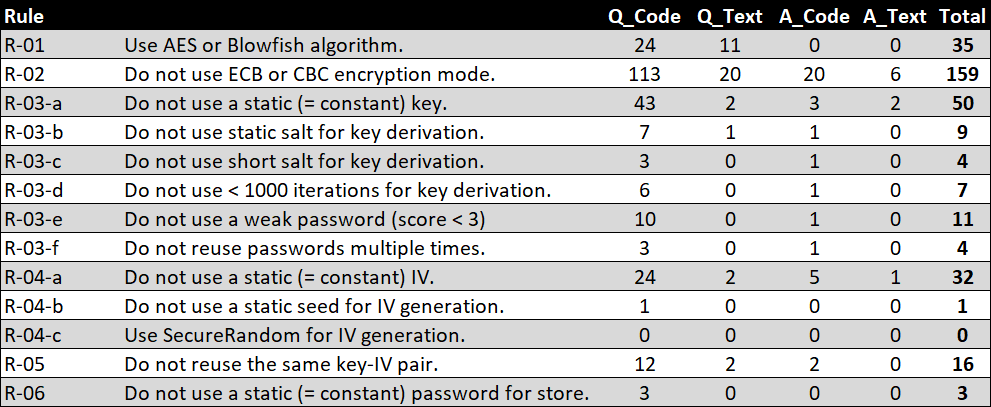
\includegraphics[width=1\textwidth]{SecTab}
\caption{Rule Violations per Check List}
\label{tab:SecRisk}
\end{table}
\par
% === Question Related Code
In the further analysis, we focused on the code snippets in the question bodies.
We did not find any additional security risks in the text or in the answers that were not present in or related to the question code.
However, some original posters only shared the code section where the issue occurred (\ie an error was thrown) and did not show how auxiliary tasks (\ie key derivation) were implemented.
We therefore must be aware that there might be even more vulnerabilities in their code.\\
On average, each question post contained 1.66 security risks in its code snippets.
We observed that the average for the most popular (and older) posts (1.91) is slightly higher than the one for the newest posts (1.43).
In total, there were 24 question posts did not contain any security risk in their code snippets.\\
The most often violated rule was \emph{R-02: Do not use ECB or CBC encryption mode}. 
In more than 75\% of question posts, the original poster used one of these unsafe block cipher modes.
This is also due to ECB being the default encryption mode for most providers.\\
The second and third most violated rules were \emph{R-03-a: Do not use a static (= constant) key.}, \emph{R-04-a: Do not use a static (= constant) IV.} and \emph{R-01: Use AES or Blowfish algorithm}. 
The number of posts using an unsafe algorithms is due to sample: We included 24 posts where DES or 3DES was used.
Some original posters stated that they used static values only for Stack Overflow to simplify their code.
Nevertheless, this is a potential security risk if we think of a programmer naively copy-pasting the code snippet.
If an original poster used both, static key and IV, this led to the reuse of key-IV pairs (\emph{R-05}) which is the fifth most often violated rule.\\
The remaining rules were rarely violated.
However,total number of rule violations referring to password based key derivation \emph{R-03-b to R-03-f} is 29.
14 posts used an unsafe key derivation procedure.
They often just hashed the password and used the first $n$ bits\footnote{$n=$ key size} instead of using a safe key derivation function such as PBKDF2.\\
The least violated rules were {R-04-c: Use SecureRandom for IV generation}, {R-04-b: Do not use a static seed for IV generation}, and {R-06: Do not use a static (=constant) password for store}.
As most original posters used ECB which does not require an IV and many used a static initialization vector otherwise, there were not many code sections showing IV generation.
There were also hardly any question posts that showed or explained how the key was stored.

% === Documentation ===
\section{Documentation}
\label{cha:ResDoc}
We were able to reduce the issues and security risks from the previous finding to 64 questions: 43 for documentation and 21 more general ones.
After checking the documentation, 10 questions remained unanswered and for 15 questions, we considered the answer as incomplete, unclear, or even misleading.\\

\subsection{Questions}
Our first observation regarding the questions was that there are twice as many JCA-specific questions as general ones.
Yet, the total priority of all "general" questions was much higher than the total priority of the specific ones even before correcting the priority for the security relevant ones.
This strongly indicates that programmers asking questions on Stack Overflow do not only lack knowledge about the JCA library but also about cryptography in general.\\

\par
The results from the first analysis gave us insight into what tasks and requirements programmers are struggling with.
The JCA-specific questions helped us to detect API related issues.\\
Several questions targeted a specific platform or were related to providers, two of them were even among the three most prioritized questions for documentation. 
As an example, the default values and behavior of a \lstinline|Cipher| object depends on the provider. 
However, whether a provider is available or not and which provider is used by default depends on the platform.
This decreases the portability of an application, in particular if the code relies on default behavior.\\
Another 5 questions were related to method overloads. 
There are two methods that perform the data transformation and both of them are overloaded.
The methods for instantiation and initialization are overloaded as well.\\
The questions also revealed that programmers particularly struggled with password based key derivation.\\
\begin{table}[h]
\centering
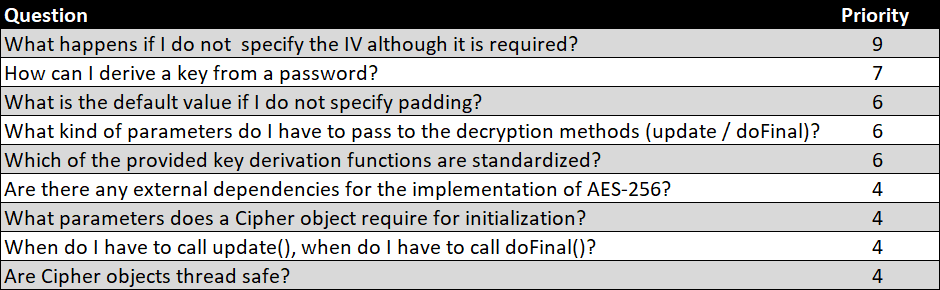
\includegraphics[width=1\textwidth]{QuestionsToDoc}
\caption{Top 9 JCA-Specific Questions}
\label{tab:Ques}
\end{table}
\par
The general questions helped us to understand what knowledge the original posters were missing.
As we only knew the accurate number for questions / issues referring to the security of code, most of the higher prioritized questions also referred to that topic.
As shown in table \ref{tab:QuesGen}, the remaining higher prioritized questions targeted the various dependencies.
We concluded that some original posters were not aware of cryptography at all.\\

\begin{table}[h]
\centering
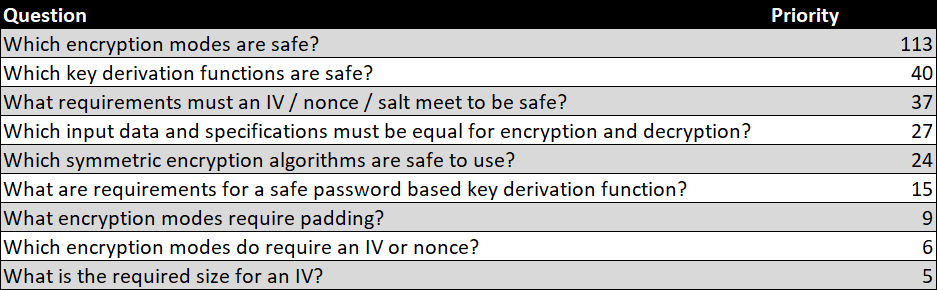
\includegraphics[width=1\textwidth]{GenQues}
\caption{Top 9 General Questions}
\label{tab:QuesGen}
\end{table}

\newpage
Among the questions that did not relate to security nor to the dependencies, we found the following topics:
\begin{itemize}
    \item AES algorithm (4 questions, total priority = 9)
    \item initialization vector (1, 4)
    \item use cases that symmetric encryption should be used for (1, 3)
    \item cipher text input for decryption (1, 2)
    \item padding (2, 2)
    \item message authentication (2, 2)
\end{itemize}

\subsection{Missing and Unclear Answers}
We were not able to find and answer to 3 JCA-specific and 7 general questions.
Most of them had a rather low priority ($<$ 4).
The higher prevalence of unanswered general questions implied that JCA documentation did not provide (enough) links to trusted resources for general information about cryptography.
There were some explanations within documentation but they were not detailed.
The following three unanswered questions represented further documentation related issues that violate the principles and recommendations described in section \ref{cha:DocQuality}):\\
\begin{itemize}
		\item \emph{Which symmetric encryption algorithms are safe to use?}
					First of all, this was the only higher prioritized question (24) that was left unanswered.
					It can be seen as an example for JCA documentation not providing enough hints regarding security.
					The reference guide mentions that ECB is not safe.
					However, it does not give any advice on what encryption mode should be used.
					What's more, there are not any further security warnings for other aspects (\ie algorithm, password based key derivation).
	\item \emph{How to specify PKCS\#7 padding in Java?}
					PKCS\#7 is a standardized padding for arbitrary block sizes that is supported by many cryptography libraries.
					JCA internally interprets PKCS\#5 padding as PKCS\#7 if it is required.
					However, this is not mentioned in the Standard Algorithm Name Specification nor in any other document that we examined.
					This might complicate the implementation of interoperability scenarios.
	\item \emph{What properties does AES-256 require?}
					There is a link to the official specifications for most algorithms in the Standard Algorithm Name Specification.
					However, for AES there is not.
					This is problematic since AES is one of only two symmetric encryption algorithms that are recommended.
					What's more, specifications are rather hard to understand.

\end{itemize}

\par
For 13 JCA specific questions and 2 more general ones, we considered the answers as not clear enough.
They often referred to method overloads. 
The documentation did not point out the differences clearly enough, it rather seemed like copy pasted.\\
\par
Another common issue was that there were not any code example for some common or important scenarios (e.g using a \lstinline|KeyStore| or password based key derivation using PBKDF2).
The available ones often did not work due to some missing parts.
In example, the code section for \lstinline|Cipher| class did not show how the algorithm parameters were generated and only demonstrated how the \lstinline|Cipher| class was used.
There were code sections later that showed how a key was randomly generated or how password based encryption could be implemented.
However, there were hardly any examples that worked all by themselves. 
\begin{figure}[h]
\centering
\includegraphics[width=0.9\textwidth]{ex2\_2}
\caption{Extract From \emph{Example 2-2 Sample Code for Using an AES Cipher with GCM Mode} \cite{javaReferenceGuide}}
\label{fig:Ex}
\end{figure}



% === D I S C U S S I O N ===
\chapter {Conclusions and Future Work}
\label{cha:Conclusion}
In this chapter, we first aim to answer our research questions based on our finding from the previous chapter.
We then discuss possible limitations of our study and suggest further research topics.\\

\par{RQ 1}: \emph{What issues do programmers face when implementing symmetric encryption using Java Cryptography Architecture?}\\
Our study provided answers to this question from different perspectives:\\
If we think of \emph{tasks} that programmers are struggling with, most of them faced problems with generating algorithm parameters, especially with deriving the key from a password.
The second most problematic task was instantiating a \lstinline|Cipher| object. 
The original posters particularly failed to specify encryption mode and padding correctly.
The third most problematic task was initializing the \lstinline|Cipher| object.
Most issues and questions related to this tasks referred to the programmer not passing all required parameters to the \lstinline|init(...)| method.\\
Another aspect was the \emph{design} of JCA library.
One of the major issues in this context was that default behavior and values depended on the provider.
The platform however determines which providers are available and what provider is chosen by default.
This decreases the portability of applications.
Another issue was that several key methods are overloaded, particularly \lstinline|getInstance(...)| and \lstinline|init(...)|.
Additionally, there are two methods that perform transformation, \lstinline|update(...)| and \lstinline|doFinal(...)| which are both overloaded as well.
Some original posters failed to chose the correct one.\\
This could also be related to the \emph{documentation}.
The method overloads are documented too similarly and there is not any advice which overload should be used in what scenario.
Also, there are not enough working code examples and it does not link to trusted, understandable resources for more general information about cryptography.\\
When we think of the \emph{programmers}, our study added more evidence confirming the assumption that they lacked knowledge about cryptography.\\


\par{RQ 2}: \emph{What are common security risks in code and advice shared on Stack Overflow referring to the implementation of symmetric encryption scenarios using JCA library?}\\
We found that security risks were particularly present in code snippets from the question body. 
Some answers gave advice or even improved security whereas others only focused on the functionality of the code.
We also observed a slight improvement when we compared the older question posts with the newer ones.\\
The most common security risk was the use of an unsafe encryption mode.
This is also related to JCA using ECB as default block cipher mode of operation.
However, some answers suggested to use CBC instead of ECB which is not safe either.\\
Other common security risks were the use of static values for either key, initialization vector, or both.
Although some original posters explicitly stated that they only used them in their post to simplify the code section, it would become a security risk if some other person just copy-pasted it.\\
The procedures used for password based key derivation also contained security risks.
JCA supports PBKDF2 as a safe procedure for password based key derivation.
However, it was rarely used.\\


\par{RQ 3}: \emph{To what extent are these issues linked to missing or inadequate documentation?}
This research question is the most difficult one to answer.
We considered most questions ($>$60\%) as clearly answered by the documentation, especially the higher prioritized ones.
We found related information for almost 85\%.
We therefore cannot blame insufficient documentation for the struggles of developers.\\
There are several explanations:
Of course it is possible that some original posters did not consult the documentation at all.
However, JCA's documentation spreads over several documents and finding a required piece of information might be time consuming.
Another explanation is that some programmers lacked the domain knowledge to understand the documentation.
As an example, if one has to derive a key from a password, he or she must know what "salt" and "iteration count" are used for and what requirements the values must meet to be safe.\\
Based on our findings, we suggest the following improvements:
\begin{itemize}
    \item Link comprehensible resources for more information about cryptography.
    \item Provide working code examples that cover all important scenarios, in particular "state of the art" scenarios (\ie authenticated encryption, password based key derivation). 
    These examples should be found in one place.
    \item Give more advice regarding security. Warn from unsafe values.
    \item In the API documentation, document method overloads more specifically, \ie describe in what scenarios which overload should be used.
\end{itemize}


\section{Limitations and Future Work}
As this project followed a qualitative approach and performed an in-depth analysis, it is reasonable to have a limited scope.
However, we found new issues that were specific for JCA library. Future work should extend it by examining more use cases and libraries.\\

\par
When it comes to the methodical approach, a major threat to validity is that we did not verify the intercoder reliability of our issue classification or our security check.
It requires a certain expertise in cryptography and software security as well as experience with JCA library. 
We did therefore not succeed in finding a suitable reviewer.
Our data is however published on GitHub\footnote{\colorbox{yellow}{ToDo}} and reanalyses are welcome.
Another limitation is that the population of Stack Overflow threads matching our scope cannot be described exactly.
There is no guarantee that the used queries returned all posts referring to our scope.
Additionally, we had to exclude almost $\frac{2}{3}$ of all threads as they did not refer to our scope.
The sample can therefore not be considered as representative for the threads referring to our scope nor for the threads returned by our queries.
This implies that the results must be verified with further investigations.\\
\par
This might also indicate that the original posters of these posts did not only struggle with cryptographic APIs when they implement a cryptography scenario. 
An important research field could be to investigate the various backgrounds of programmers and develop tools that support them in acquiring knowledge about computer science in general as well as more specific topics such as cryptography.\\
\par
Software security requires expertise, especially while working with a low-level library such as JCA.
Not all programmers working in a security context however have the required domain knowledge.
Security should therefore be an essential part in the education of future software developers.
But also the IT industry must be aware of the importance of security and how difficult it is.
Researchers must find ways to put their findings and tools into practice.





% === A N L E I T U N G   Z U   W I S S E N S C H A F T L I C H E M   A R B E I T E N
\chapter {Anleitung zu wissenschaftlichem Arbeiten}
\label{cha:AWI}
One obstacle that we observed during the thesis project was that JCA documentation did not contain enough working code examples.
We therefore decided to provide a best-practice example for password based encryption (PBE) which is a common use case.\\
Unlike the PBE example in the JCA Reference Guide \cite{javaReferenceGuide}, our example does not rely on the default behavior.
This allows us to use of GCM encryption mode which is the recommended block cipher mode of operation (\ie Nakov \cite{nakov2018}).\\
\par
The example is also available on GitHub\footnote{\colorbox{yellow}{ToDo}}.
It illustrates the encryption of \lstinline|String| objects and files.
It can be used as a service class for \textit{educational purpose}.
A guide on how to use it can be found in the corresponding \href{}{ReadMe} file.%ToDo
\begin{figure}[h]
    \centering
    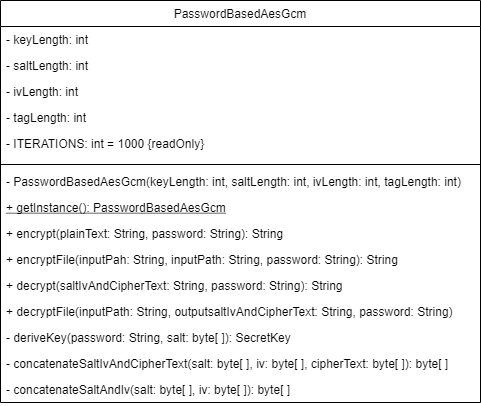
\includegraphics[width=0.8\textwidth]{Anleitung/UML}
    \caption{UML of the Example Service Class Showing the Most Important Class Variables and Methods}
    \label{fig:UML}
\end{figure}
The code should work if any providers are available that support the \lstinline|Cipher|-transformation "AES/GCM/NOPADDING" and the key derivation function "PBKDF2WithHmacSHA256".
We built and tested the implementation on Java 15.0.1 using the default SunJCE Provider (version 15) for both, \lstinline|Cipher| and \lstinline|SecretKeyFactory| class.\\

\newpage
\par
The aim of this chapter is to explain our example code.
It describes and justifies each implementation step and also provides the most important security hints.
We sometimes make use of class variables, namely the lengths of various algorithm parameters as well as the number of iterations performed during key derivation.\\
Depending on the kind of application, they could all be constants (such as \lstinline|ITERATIONS|). 
We kept them modifiable because we wanted to support a wider range of use cases.\\
Figure \ref{fig:params} shows the class variables used in our example. 
The comments indicate what values acceptable to have both, a functioning and a secure application.
\begin{figure}[h]
    \centering
    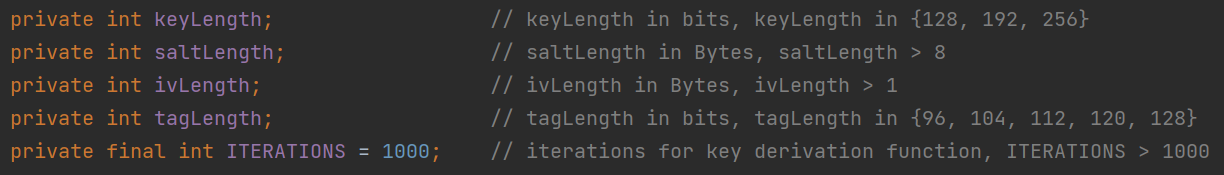
\includegraphics[width=1\textwidth]{Anleitung/genParams}
    \caption{Class Variables and Their Constraints}
    \label{fig:params}
\end{figure}

\newpage
\section{Subroutines}
\subsection*{\lstinline|deriveKey(String password, byte[] salt)|}
\begin{figure}[h]
    \centering
    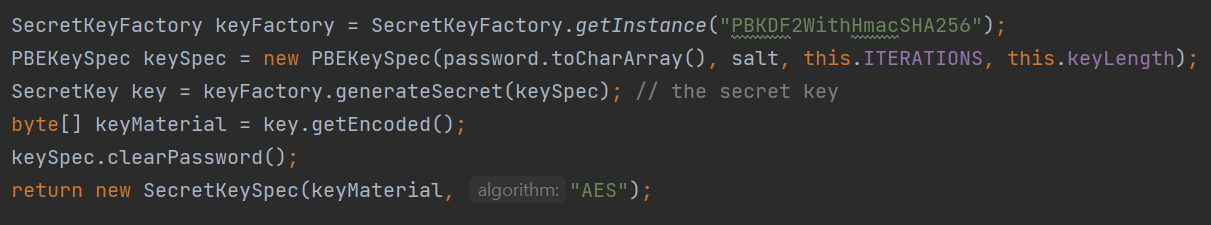
\includegraphics[width=1\textwidth]{Anleitung/keyDer}
    \caption{Algorithm for Key Derivation}
    \label{fig:keyDer}
\end{figure}
This is probably the most crucial task of the implementation.
As we want to derive the key from a password, we must instantiate a \lstinline|SecretKeyFactory| object using a password based key derivation function as algorithm.
We selected "PBKDF2WithHmacSHA256" as is both, secure and standardized. It is therefore also suitable for scenarios where different platforms are involved.
PBKDF2 can also be used with another pseudo random function (\ie HmacSHA1), depending on the specification of the other platform.\\
We then must instantiate a \lstinline|PBEKeySpec| that holds the password, the salt, the number of iterations as well as the length of the key.
We can use the \lstinline|keyFactory| to generate a \lstinline|SecretKey|from the \lstinline|PBEKeySpec|.\\
However, the factory transmits its algorithm to the generated key.
But to use it with an "AES"-\lstinline|Cipher| object, the key must hold "AES" as algorithm as well.
We worked around this issue by fetching the key material from the generated key (\lstinline|getEncoded()|) and instantiate a new one holding "AES" as algorithm.
Since \lstinline|SecretKey| is an interface, we instantiated a \lstinline|SecretKeySpec| instead.\\

\par
Additionally to the statements shown in figure \ref{fig:keyDer}, the method includes some minimal error handling. To have a safe application it is important to
\begin{itemize}
    \item use a safe password
    \item use a safe key derivation function
    \item use random salt of at least 64 bits (8 Bytes).
    \item clear the password from the \lstinline|PBEKeySpec| after generating the (first) key.
\end{itemize}

\newpage
\subsection*{\lstinline|concatenateSaltIvAndCipherText(byte[] salt, byte[] iv, byte[] cipherText)|}
\begin{figure}[h]
\centering
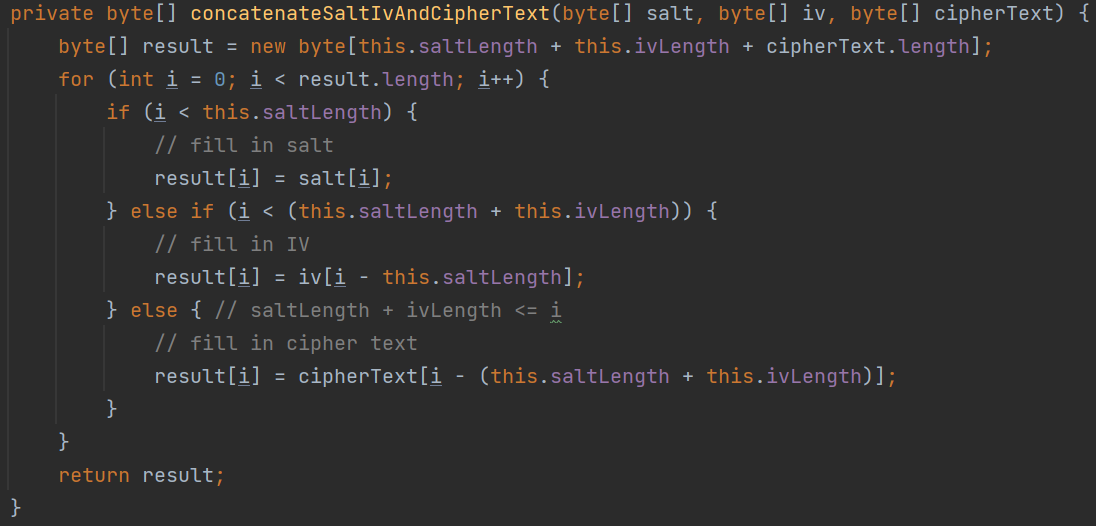
\includegraphics[width=1\textwidth]{Anleitung/concat}
\caption{Subroutine to Concatenate Salt, Initialization Vector, and Cipher Text}
\label{fig:concat1}
\end{figure}
Since encryption and decryption must use the same salt and initialization vector (IV), we have to transmit these values from the encryptor to the decryptor.
However, they must not remain secret.
We therefore decided to prepend these values to the cipher text when encrypting a \lstinline|String|.
As a \lstinline|Cipher| object returns the cipher text as a \lstinline|byte| array, we just have to create a larger byte array and correctly copy the values.

\subsection*{\lstinline|concatenateSaltAndIvA(byte[] salt, byte[] iv)|}
Similarly to the previous subroutine, this method joins two \lstinline|byte| arrays. Since we are not returning any cipher text when encrypting a file, we only want to return the salt and the IV.




\newpage
\section{Encryption}
\label{cha:Enc}
\subsection*{Configuring the Cipher Object}
Whether we are encrypting a \lstinline|String| or a file, we need to instantiate and initialize a \lstinline|Cipher| object.
The following lines of code are therefore part of both encryption methods, \lstinline|encrypt(...)| and \lstinline|encryptFile(...)|.
\vspace{3mm}\\
The first thing we must do is creating the required algorithm parameters.
After generating some random \lstinline|byte| values for salt using a \lstinline|SecureRandom| object, we can call the previously described subroutine to derive a key from our password.
Since we are using GCM encryption mode, we also require a \lstinline|GCMParameterSpec| object.
It holds the length of the authentication tag (\lstinline|tagLength|) and a randomly generated IV.
\begin{figure}[h]
    \centering
    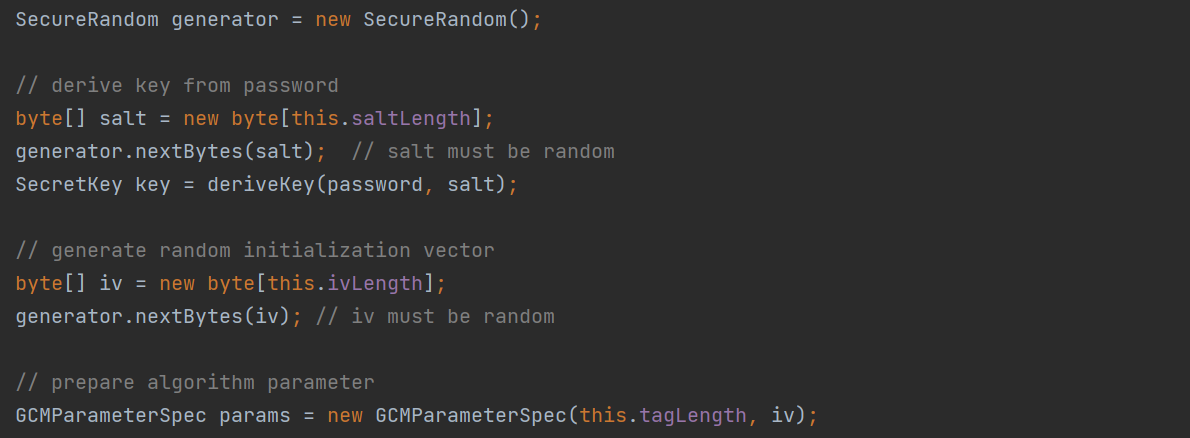
\includegraphics[width=1\textwidth]{Anleitung/gen_params_1}
    \caption{Generating a \lstinline|SecretKey| and \lstinline|GCMParameterSpec|}
    \label{fig:gp1}
\end{figure}\\
Then we can instantiate the \lstinline|Cipher| object and pass the parameters using the \lstinline|init(...)| method.
\begin{figure}[h]
    \centering
    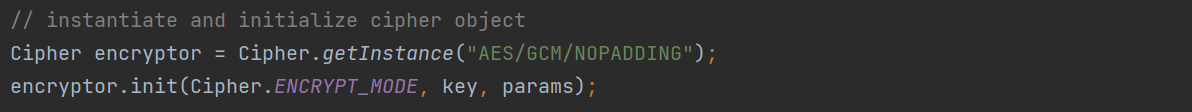
\includegraphics[width=1\textwidth]{Anleitung/init_enc}
    \caption{Instantiating and Initializing a \lstinline|Cipher| Object for Encryption}
    \label{fig:init_enc}
\end{figure}\\

\newpage
\subsection*{Encrypting a String\\ 
\lstinline|encrypt(String plaintext, String password)|}
% Character Decoding
Since encryption is performed on bytes, we must convert the plain text into a \lstinline|byte| array.
This can be done using \lstinline|String|'s \lstinline|getBytes()| method.
To ensure interoperability and portability, we recommend to specify the character set (\ie UTF-8) that should be used for decoding.\\
\begin{figure}[h]
    \centering
    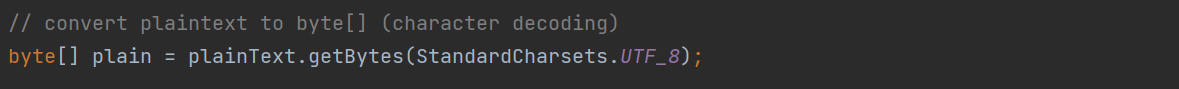
\includegraphics[width=1\textwidth]{Anleitung/decoding_1}
    \caption{Converting Plain Text to \lstinline|byte[]|: Character Decoding}
    \label{fig:dec1}
\end{figure}\\
The resulting \lstinline|byte| array is passed to \lstinline|Cypher|'s \lstinline|doFinal(...)| method that performs encryption.
\begin{figure}[h]
    \centering
    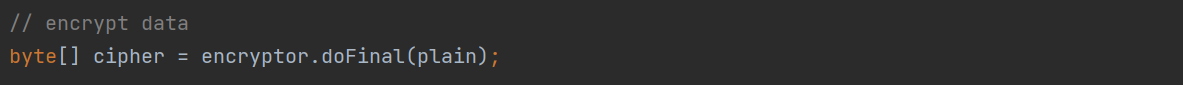
\includegraphics[width=1\textwidth]{Anleitung/enc_string}
    \caption{Encrypting Plain Text}
    \label{fig:dec1}
\end{figure}\\
As previously mentioned, we want to transmit the salt and the IV along the cipher text.
To do so, we prepend them to the encryption result.
After joining the three arrays, we want to convert it back into a \lstinline|String|.
Each of the concatenated values potentially contains any bit sequence, also sequences that are not included in a standard character. 
We must therefore use base64 encoding as we might lose data otherwise.
\begin{figure}[h]
    \centering
    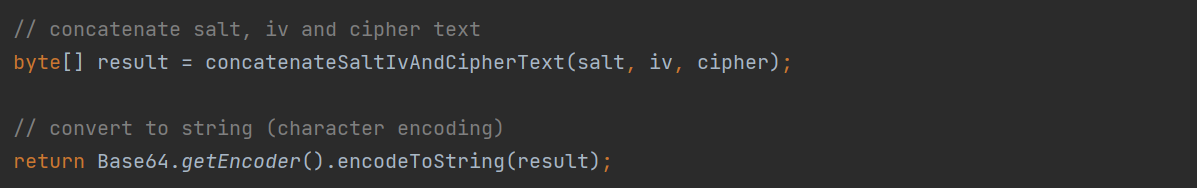
\includegraphics[width=1\textwidth]{Anleitung/transmission}
    \caption{Encrypting Plain Text}
    \label{fig:dec1}
\end{figure}\\



\newpage
\subsection*{Encrypting a File\\
\lstinline|encryptFile(String inputPath, String outputPath, String password)|}
The first things we need to do is opening a set of streams: 
\begin{itemize}
    \item a \lstinline|FileInputStream| to read from the file specified by \lstinline|inputPath|
    \item a \lstinline|CipherInputStream| that encrypts anything read by the \lstinline|FileInputStream| using the previously initialized \lstinline|Cipher| object
     \item a \lstinline|FileOutputStream| that writes the encryption results to the \lstinline|outputPath|
\end{itemize}
\begin{figure}[h]
    \centering
    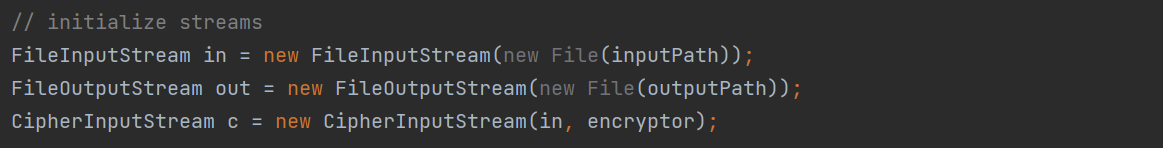
\includegraphics[width=1\textwidth]{Anleitung/init_streams_enc}
    \caption{Initializing Streams for File Encryption}
    \label{fig:init_streams_1}
\end{figure}
The streams can now be used to read and encrypt the file block wise. 
To do so, the \lstinline|CipherInputStream| must read (and encrypt) the next block of bytes and store it to an int variable.
The value is then written to the output file by the \lstinline|FileOutputStream|.\\
\begin{figure}[h]
    \centering
    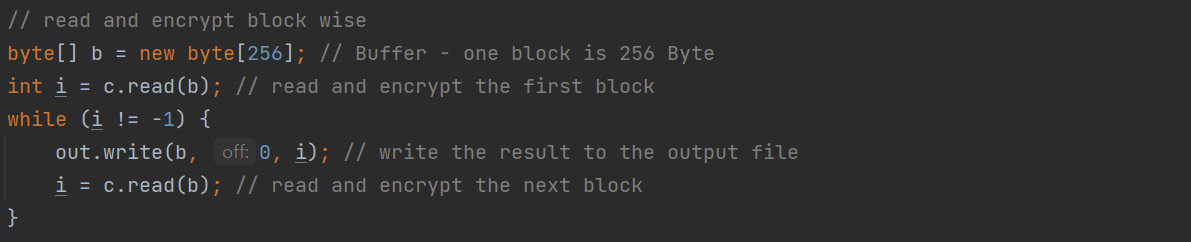
\includegraphics[width=1\textwidth]{Anleitung/enc_streams}
    \caption{Using Streams to Encrypt the Content of a File Block Wise}
    \label{fig:enc_streams}
\end{figure}\\
When the streams are done, we must close them.\\
\begin{figure}[h]
    \centering
    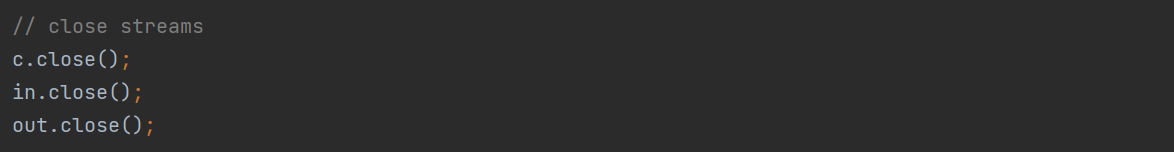
\includegraphics[width=1\textwidth]{Anleitung/close_streams}
    \caption{Closing all Streams}
    \label{fig:close}
\end{figure}\\
Similarly to the encryption result from encrypting a \lstinline|String|, we are returning the salt and the IV concatenated and base64 encoded.
\begin{figure}[h]
    \centering
    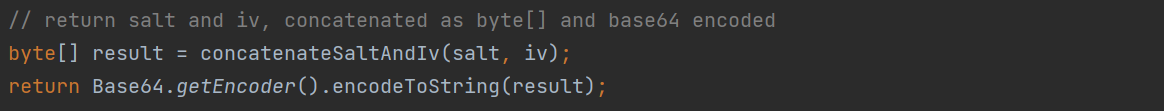
\includegraphics[width=1\textwidth]{Anleitung/trans_streams}
    \caption{Returning Base64 Encoded Salt and IV}
    \label{fig:close}
\end{figure}
\subsection*{Security Requirements for Encryption}
\begin{itemize}
    \item Use a safe algorithm (AES or Blowfish).
    \item Use a safe block cipher mode of operation (preferably CTR or GCM). 
    \item Use a safely derived, secret key.
    \item Use a random initialization vector that was generated using a secure source of randomness (\ie \lstinline|SecureRandom|).
    \item Use a new key-IV pair each time you perform encryption.
\end{itemize}
\newpage
\section{Decryption}
\label{cha:Dec}
\subsection*{Decrypting a String\\
\lstinline|decrypt(String saltIvAndCipherText, String password)|}
As we base64 encoded the encryption result, we first must decode it using the same format.\\
\begin{figure}[h]
    \centering
    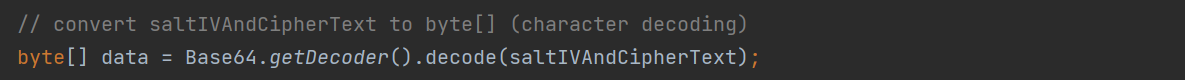
\includegraphics[width=1\textwidth]{Anleitung/decoding_2}
    \caption{Base64 Decoding}
    \label{fig:trans}
\end{figure}\\
% Restoring Parameters
Next, we must restore the parameters.
As we prepended the salt and the IV to the cipher text, they can easily be restored using \lstinline|saltLength| and \lstinline|ivLength| class variables.
We can then derive the key using the password parameter and the retrieved salt and instantiate another \lstinline|GCMParameterSpec| using the \lstinline|tagLength| class variable and the retrieved IV.\\
\begin{figure}[h]
    \centering
    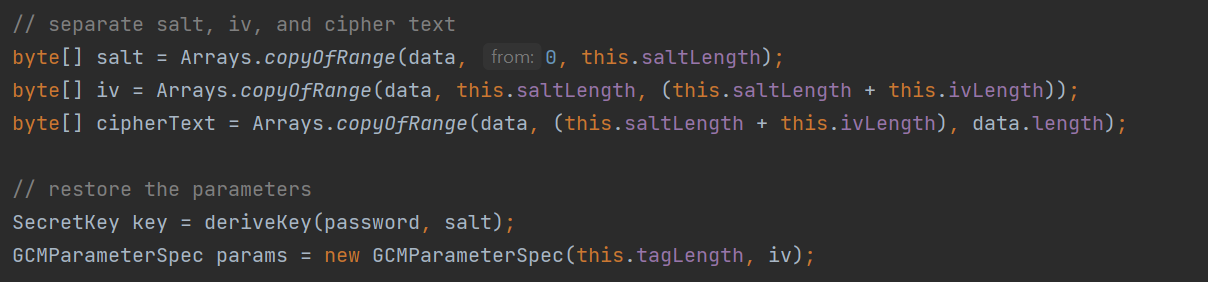
\includegraphics[width=1\textwidth]{Anleitung/gen_params_2}
    \caption{Restoring Algorithm Parameters}
    \label{fig:params2}
\end{figure}\\
Finally we can instantiate and initialize another \lstinline|Cipher| object and ask it to decrypt the cipher text.\\
\begin{figure}[h]
    \centering
    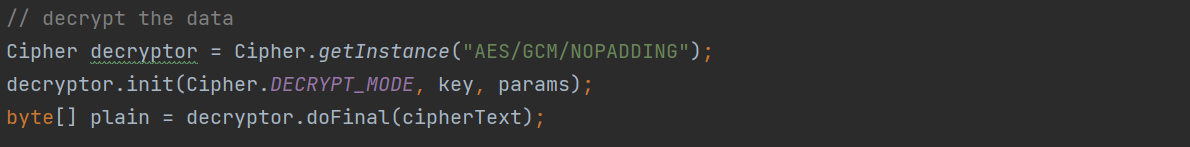
\includegraphics[width=1\textwidth]{Anleitung/decryption}
    \caption{Instantiating and Initializing a \lstinline|Cipher| Object and Asking It for Decryption}
    \label{fig:decryption}
\end{figure}\\
In the end, we just have to convert the \lstinline|byte| array holding the plain text back to a \lstinline|String| using the same character set that was used for decoding it before encryption (\ie UTF-8).
\begin{figure}[h]
    \centering
    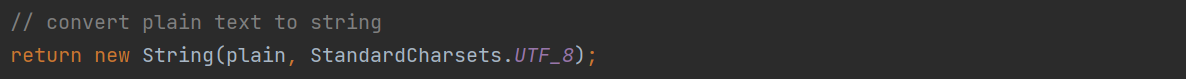
\includegraphics[width=1\textwidth]{Anleitung/encoding}
    \caption{Character Encoding the Plain Text}
    \label{fig:encoding}
\end{figure}



\newpage
\subsection*{Decrypting a File\\
\lstinline|decryptFile(String inputPath, String outputPath, String saltAndIv, String password|}
Similarly to \lstinline|String| decryption, we first must restore the parameters.
To do so, we base64-decode the \lstinline|saltAndIv| parameter and separate the values using the \lstinline|saltLength| and \lstinline|ivLength| class variables.
The salt is used with the password to derive the key.
The IV is passed to a new \lstinline|GCMParameterSpec| object along the \lstinline|tagLength| class variable.
Then, we can instantiate and initialize a \lstinline|Cipher| object.\\
\begin{figure}[h]
    \centering
    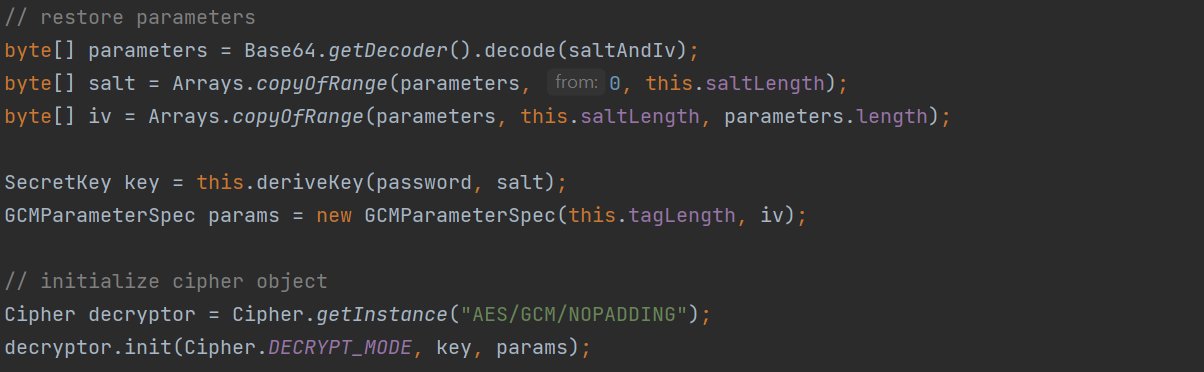
\includegraphics[width=1\textwidth]{Anleitung/restore_streams}
    \caption{Restoring the Algorithm Parameters for File Decryption and Creating a \lstinline|Cipher| Object}
    \label{fig:restore_stream}
\end{figure}\\
The rest of the decryption is implemented in the exact same way as encryption:
\begin{enumerate}
    \item Open a \lstinline|FileInputStream|, a \lstinline|CipherInputStream|\footnote{use the prepared \lstinline|decryptor| instead of an encrypting \lstinline|Cipher| object}, and a \lstinline|FileOutputStream| (see figure \ref{fig:init_streams_1}).
    \item Block wisely read (and decrypt) the input file using the \lstinline|CipherInputStream| and write the result to the output file using the \lstinline|FileOutputStream| (see figure \ref{fig:enc_streams})
    \item Close the streams (see figure \ref{fig:close})
\end{enumerate}
As the plain text has already been written to the output file, this method does not have a return value.



\newpage
\section{Some Remarks on Parameter Transmission}
We did not include any form of parameter transmission or storage in our example because this aspect strictly depends on the kind of application.
In client-server scenarios we might need to transmit the parameters via HTTPS.
In some scenarios it is sufficient to store them locally.\\
\par
However, we want to emphasize the importance of keeping the password a secret. 
It is the only value not known by a potential intruder.
If one needs to store or transmit it, it should be wrapped using (public key) encryption\\
\par
In case of customized algorithm parameter lengths (class variables), these must also be stored to ensure that all parameters can be restored at decryption.
Our example class provides a simple, static \lstinline|getInstance()| method to create a valid default \lstinline|PasswordBasedAesGcm| object.
However, there are setter methods to customize the class variables.
They can be retrieved by calling the corresponding getter methods.
The values may be transmitted as separate \emph{POST} variables or stored in a database along the encryption result.
\begin{figure}[h]
    \centering
    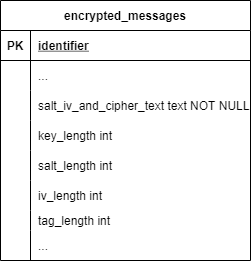
\includegraphics[width=0.5\textwidth]{Anleitung/DB}
    \caption{Draft of a Database Entity}
    \label{fig:params}
\end{figure}






% === B I B L I O G R A P H Y ===
\bibliography{thesis}
\bibliographystyle{plain}


% === A P P E N D I X ===
\chapter*{Appendix}
\section*{A \hspace{5mm} Sample and Analysis Related Data}
\newpage
All data related to 
\section*{B \hspace{5mm} Reasons for Excluding Threads During Sampling}
\label{App:B}
\begin{itemize}
	\item \textbf{too general}: posts referring to cryptographic concepts or cyber security in general rather than the targeted API\\ 
			\emph{Example: \href{https://stackoverflow.com/questions/21732018/how-to-check-if-a-string-is-encrypted-or-not}{How to check if a string is encrypted or not?}}

	\item \textbf{does not refer to cryptography}: issues occurring in a non-cryptographic context, i.e. establishing a network connection or file access\\
			\emph{Example: \href{https://stackoverflow.com/questions/1755259/syntax-error-on-token-expected-after-this-token}{Syntax error}}

	\item \textbf{does not refer to symmetric encryption}: posts referring to other cryptographic concepts such as asymmetric encryption or hashing\\
			\emph{Example: \href{https://stackoverflow.com/questions/66941359/rsa-decryption-fails}{RSA decryption (fails)}} 

	\item \textbf{does not refer to JCA}: issues occurring during a symmetric encryption scenario but which are not due to Java Cryptography Architecture.
				Such issues can refer to another library (e.g. BouncyCastle) or to some other aspect such as character encoding.\\
				\emph{Example: \href{https://stackoverflow.com/questions/5641326/256bit-aes-cbc-pkcs5padding-with-bouncy-castle}{256bit AES/CBC/PKCS5Padding with Bouncy Castle}}

	\item \textbf{does not refer to targeted algorithm}: posts referring to other algorithms than the targeted ones\\
			\emph{Example: \href{https://stackoverflow.com/questions/62721499/decryption-using-blowfish-failing}{Decryption using blowfish failing}}

	\item \textbf{looking for an equivalent} or \textbf{interoperability issue}:  looking for equivalents / counterparts in different programming languages\\
			\emph{Example: \href{https://stackoverflow.com/questions/19698721/encrypt-in-node-and-decrypt-in-java}{Encrypt in node and decrypt in java}} 

	\item \textbf{negative votes} or \textbf{closed}: posts of poor quality

	\item \textbf{academic}: posts with a different focus than obstacles when using the API

	\item \textbf{duplicate}: Duplicates are often left unanswered (or only answered with the reference to a similar post). For posts belonging to the "most popular" category, we included a duplicate if it had more views than the original.
\end{itemize}


\newpage
\section*{C \hspace{5mm} Example Records For Issue Classification}
\subsection*{Technical Aspects}
\begin{tabular}{|m{0.15\textwidth}|m{0.25\textwidth}|m{0.22\textwidth}|m{0.28\textwidth}|}
\hline
    \footnotesize Category&
    \footnotesize Issue&
    \footnotesize Reason&
    \footnotesize Solution\\
\hline
\hline
    \scriptsize Algorithm&
    \scriptsize TripleDES vs. DESede - what is the difference?&
    -&
    \scriptsize They are equivalent. TripleDES is the name for SunJCE
                Provider\\
\hline
    \scriptsize Encryption Mode&
    \scriptsize Convert AES-128-CBC PHP to Java&
    \scriptsize different encryption modes \newline 
                (CBC vs. Java default = ECB)&
    \scriptsize Use "AES/CBC/PKCS5PADDING"\\
\hline
    \scriptsize Padding&
    \scriptsize Why does doFinal() add extra bytes to my cipher text?
                How can I remove them?&
    -&
    \scriptsize doFinal() adds padding for block ciphers.
                It is removed automatically if the same padding is specified for en- and decryption\\
 \hline
    \scriptsize Dependency Encryption Mode - Padding&
    \scriptsize IllegalBlockSizeException : \newline
    Input length must be multiple of 16 when decrypting with padded cipher&
    \scriptsize Transformation "AES" might be interpreted as "AES/ECB/NoPadding". \newline
    ECB is a block cipher and requires padding in most cases&
    \scriptsize add padding or switch encryption mode\\
\hline
    \scriptsize Cipher Object \newline 
                Instantiation - Other&
    \scriptsize NoSuchAlghoritmExeption for "AES/ECB/PKCS5Padding" on Android&
    -&
    -\\
\hline
\hline
    \scriptsize Key Derivation&
    \scriptsize InvalidKeyException: Invalid AES key length: 128 bytes&
    \scriptsize Key retrieved through Diffie-Hellman is 128 Bytes instead of bits&
    \scriptsize Generate key of correct size\\
\hline
    \scriptsize IV / Nonce \newline Generation&
    \scriptsize invalid IV length&
    \scriptsize IV = [00000000000000000] \newline
    $\rightarrow$ length = 1&
    \scriptsize IV = [0,0,0,0,0,0,0,0,0,0,0,0,0,0,0,0] \newline $\rightarrow$ length = 16\\
\hline
    \scriptsize Generation of Other Algorithm \newline Parameters&
    \scriptsize AES-GCM: different output for AuthenticationTag for Java and JS&
    \scriptsize Using Timestamp as AAD&
    -\\
\hline
\hline
    \scriptsize Dependency \newline
    Algorithm - Key&
    \scriptsize Is this code AES-256 encryption?&
    -&
    \scriptsize Yes, key is of size 256b\\
\hline
    \scriptsize Dependency Algorithm/Encryption Mode - IV&
    \scriptsize InvalidKeyException: Parameters missing (IV)&
    \scriptsize CBC requires IV&
    \scriptsize add IV or switch encryption mode\\
\hline
    \scriptsize Cipher Object Initialization - Other&
    \scriptsize How is the IV generated (if it is not passed to Cipher.init())?&
    -&
    \scriptsize default values depend on provider\\
\hline
\hline
    \scriptsize Transformation&
    \scriptsize BadPaddingException: pad block corrupted&
    \scriptsize you shouldn't call doFinal() on every block, because doFinal() expects any padding at the end, which obviously won't be there in intermediate blocks&
    \scriptsize Either (a) call update() on intermediate data, then doFinal() at the end, or (b) just arrange to have all your data in one buffer or byte array, and call doFinal() once on the whole job lot.\\
\hline
\hline
    \scriptsize Key Transmission&
    \scriptsize Stored tat DES Secretkey into database converting it into String. Now i want to Convert that String to Secretkey.&
    -&
    \scriptsize You are seeing the object class and the hashcodes of 2 different instances sharing the same reference. If you want to confirm whether your key is getting decoded correctly, print the encoded version of the decoded key.\\
\hline
    \scriptsize Transmission of Other Algorithm Parameters&
    \scriptsize how to decrypt cipher text encrypted with salt&
    -&
    \scriptsize pass salt along cipher text\\
\hline
\hline
    \scriptsize Dependency Encryptor - Decryptor&
    \scriptsize BadPaddingException: Given final block not properly padded&
    \scriptsize OP generates new key for decryption&
    \scriptsize pass encryption key to decryption section as parameter\\
\hline
\end{tabular}
\newpage
\subsection*{Requirements}
\begin{tabular}{|m{0.15\textwidth}|m{0.25\textwidth}|m{0.22\textwidth}|m{0.28\textwidth}|}
\hline
    \footnotesize Category&
    \footnotesize Issue&
    \footnotesize Reason&
    \footnotesize Solution\\
\hline
\hline
    \scriptsize Use Case&
    \scriptsize inappropriate use case&
    \scriptsize OP want to store password encrypted&
    \scriptsize store hash instead\\
\hline
    \scriptsize Performance&
    \scriptsize Encryption of large file is very slow (AES)&
    -&
    -\\
\hline
    \scriptsize Space&
    \scriptsize OutOfMemoryException for large files&
    \scriptsize This appears to be an issue with the implementation of the GCM mode. I'm not sure that you can work-around it.&
    -\\
\hline
    \scriptsize Reliability&
    \scriptsize Cryptograhy Service crashes about 1x/day&
    \scriptsize Cipher objects in global scope --> Cipher is not thread safe&
    -\\
\hline
    \scriptsize Portability&
    \scriptsize Same code produces different cipher text on "native java" and android platform&
    \scriptsize default values depend on platform&
    \scriptsize fully specify transformation\\
\hline
    \scriptsize Interoperability&
    \scriptsize Same key generation procedure results in different keys&
    \scriptsize SHA1PRNG is not standardized&
    \scriptsize use standardized RNG\\
\hline
    \scriptsize Security&
    \scriptsize unsafe encryption mode (ECB)&
    \scriptsize default value&
    \scriptsize fully specify transformation\\
\hline
\end{tabular}
%END Doc
%-------------------------------------------------------

\end{document}